% LaTeX source for ``Think OS:
% A Brief Introduction to Operating Systems''
% Copyright 2015  Allen B. Downey.

% License: Creative Commons Attribution-NonCommercial 3.0 Unported License.
% http://creativecommons.org/licenses/by-nc/3.0/
%

%\documentclass[10pt,b5paper]{book}
\documentclass[12pt]{book}
\usepackage[width=5.5in,height=8.5in,
  hmarginratio=3:2,vmarginratio=1:1]{geometry}

% for some of these packages, you might have to install
% texlive-latex-extra (in Ubuntu)

\usepackage[T1]{fontenc}
\usepackage{textcomp}
\usepackage{mathpazo}
%\usepackage{pslatex}

\usepackage{url}
\usepackage{fancyhdr}
\usepackage{fancyvrb}
\usepackage{graphicx}
\usepackage{subfig}
\usepackage{amsmath}
\usepackage{amsthm}
%\usepackage{amssymb}
\usepackage{makeidx}
\usepackage{setspace}
\usepackage{hevea}                           
\usepackage{upquote}
\usepackage{listings}
\usepackage{color}

\title{Think OS}
\author{Allen B. Downey}

\newcommand{\thetitle}{Think OS: A Brief Introduction to Operating Systems}
\newcommand{\theversion}{0.7.2}

% these styles get translated in CSS for the HTML version
\newstyle{a:link}{color:black;}
\newstyle{p+p}{margin-top:1em;margin-bottom:1em}
\newstyle{img}{border:0px}

% change the arrows in the HTML version
\setlinkstext
  {\imgsrc[ALT="Previous"]{back.png}}
  {\imgsrc[ALT="Up"]{up.png}}
  {\imgsrc[ALT="Next"]{next.png}} 

% Commands that control the appearance of the listings
\definecolor{light-gray}{gray}{0.95}

\lstset{basicstyle=\tt, frame=single, 
backgroundcolor=\color{light-gray}, escapeinside={(*}{*)},
numbers=left, numberstyle=\tiny, numbersep=10pt}


\makeindex

\newif\ifplastex
\plastexfalse

\begin{document}

\frontmatter

\ifplastex
    \usepackage{localdef}
    \maketitle

\else

%%% EXERCISE

\newtheoremstyle{exercise}% name of the style to be used
  {\topsep}% measure of space to leave above the theorem. E.g.: 3pt
  {\topsep}% measure of space to leave below the theorem. E.g.: 3pt
  {}% name of font to use in the body of the theorem
  {0pt}% measure of space to indent
  {\bfseries}% name of head font
  {}% punctuation between head and body
  { }% space after theorem head; " " = normal interword space
  {}% Manually specify head

\theoremstyle{exercise}
\newtheorem{exercise}{Exercise}[chapter]

\input{latexonly}

\begin{latexonly}

\renewcommand{\blankpage}{\thispagestyle{empty} \quad \newpage}

%\blankpage
%\blankpage

% TITLE PAGES FOR LATEX VERSION

%-half title--------------------------------------------------
\thispagestyle{empty}

\begin{flushright}
\vspace*{2.0in}

\begin{spacing}{3}
{\huge Think OS: A Brief Introduction to Operating Systems}\\
{\Large }
\end{spacing}

\vspace{0.25in}

Version \theversion

\vfill

\end{flushright}

%--verso------------------------------------------------------

\blankpage
\blankpage
%\clearemptydoublepage
%\pagebreak
%\thispagestyle{empty}
%\vspace*{6in}

%--title page--------------------------------------------------
\pagebreak
\thispagestyle{empty}

\begin{flushright}
\vspace*{2.0in}

\begin{spacing}{3}
{\huge Think OS}\\
{\Large  A Brief Introduction to Operating Systems}
\end{spacing}

\vspace{0.25in}

Version \theversion

\vspace{1in}


{\Large
Allen B. Downey\\
}


\vspace{0.5in}

{\Large Green Tea Press}

{\small Needham, Massachusetts}

%\includegraphics[width=1in]{figs/logo1.eps}
\vfill

\end{flushright}


%--copyright--------------------------------------------------
\pagebreak
\thispagestyle{empty}

{\small
Copyright \copyright ~2015 Allen B. Downey.


\vspace{0.2in}

\begin{flushleft}
Green Tea Press       \\
9 Washburn Ave \\
Needham MA 02492
\end{flushleft}

Permission is granted to copy, distribute, and/or modify this document
under the terms of the Creative Commons Attribution-NonCommercial 3.0 Unported
License, which is available at \url{http://creativecommons.org/licenses/by-nc/3.0/}.

The original form of this book is \LaTeX\ source code.  Compiling this
code has the effect of generating a device-independent representation
of a textbook, which can be converted to other formats and printed.

The \LaTeX\ source for this book is available from
\url{http://greenteapress.com/thinkos}.

The cover for this book is based on a photo by Paul Friel
(\url{http://flickr.com/people/frielp/}), who made it available under
the Creative Commons Attribution license.  The original photo
is at \url{http://flickr.com/photos/frielp/11999738/}.

\vspace{0.2in}

} % end small

\end{latexonly}


% HTMLONLY

\begin{htmlonly}

% TITLE PAGE FOR HTML VERSION

{\Large \thetitle}

{\large Allen B. Downey}

Version \theversion

\vspace{0.25in}

Copyright 2011 Allen B. Downey

\vspace{0.25in}

Permission is granted to copy, distribute, and/or modify this document
under the terms of the Creative Commons Attribution-NonCommercial 3.0
Unported License, which is available at
\url{http://creativecommons.org/licenses/by-nc/3.0/}.

\setcounter{chapter}{-1}

\end{htmlonly}

\fi
% END OF THE PART WE SKIP FOR PLASTEX

\chapter{Preface}
\label{preface}

In many computer science programs, Operating Systems is an advanced
topic.  By the time students take it, they know how to program
in C, and they have probably taken a class in Computer Architecture.
Usually the goal of the class is to expose students to the design
and implementation of operating systems, with the implied assumption
that some of them will do research in this area, or write part of
an OS.

This book is intended for a different audience, and it has different
goals.  I developed it for a class at Olin College called Software
Systems.

Most students taking this class learned to program in Python,
so one of the goals is to help them learn C.
For that part of the class, I use Griffiths and Griffiths, {\it Head
  First C}, from O'Reilly Media.  This book is meant to complement
that one.

Few of my students will ever write an operating system, but many of
them will write low-level applications in C or work on embedded
systems.  My class includes material from operating systems, networks,
databases, and embedded systems, but it emphasizes the topics
programmers need to know.

This book does not assume that you have studied Computer Architecture.
As we go along, I will explain what we need.

If this book is successful, it should give you a better understanding
of what is happening when programs run, and what you can do to make
them run better and faster.

Chapter 1 explains some of the differences between compiled and
interpreted languages, with some insight into how compilers work.
Recommended reading: {\it Head First C} Chapter 1.

Chapter 2 explains how the operating system uses processes to
protect running programs from interfering with each other.

Chapter 3 explains virtual memory and address translation.
Recommended reading: {\it Head First C} Chapter 2.

Chapter 4 is about file systems and data streams.
Recommended reading: {\it Head First C} Chapter 3.

Chapter 5 describes how numbers, letters, and other values are
encoded, and presents the bitwise operators.

Chapter 6 explains how to use dynamic memory management, and how
it works.
Recommended reading: {\it Head First C} Chapter 6.

Chapter 7 is about caching and the memory hierarchy.

Chapter 8 is about multitasking and scheduling.

Chapter 9 is about POSIX threads and mutexes.
Recommended reading: {\it Head First C} Chapter 12 and
{\it Little Book of Semaphores} Chapters 1 and 2.

Chapter 10 is about POSIX condition variables and the producer/consumer
problem. Recommended reading: {\it Little Book of Semaphores} Chapters 3
and 4.

Chapter 11 is about using POSIX semaphores and implementing semaphores in C.

\section*{A note on this draft}

The current version of this book is an early draft.  While I am
working on the text, I have not yet included the figures.  So
there are a few places where, I'm sure, the explanation will be
greatly improved when the figures are ready.


\section{Using the code}
\label{code}

Example code for this book is available from
\url{https://github.com/AllenDowney/ThinkOS}.  Git is a version
control system that allows you to keep track of the files that
make up a project.  A collection of files under Git's control is
called a {\bf repository}.  GitHub is a hosting service that provides
storage for Git repositories and a convenient web interface.
\index{repository}
\index{Git}
\index{GitHub}

The GitHub homepage for my repository provides several ways to
work with the code:

\begin{itemize}

\item You can create a copy of my repository
on GitHub by pressing the {\sf Fork} button.  If you don't already
have a GitHub account, you'll need to create one.  After forking, you'll
have your own repository on GitHub that you can use to keep track
of code you write while working on this book.  Then you can
clone the repo, which means that you copy the files
to your computer.
\index{fork}

\item Or you could clone
my repository.  You don't need a GitHub account to do this, but you
won't be able to write your changes back to GitHub.
\index{clone}

\item If you don't want to use Git at all, you can download the files
in a Zip file using the button in the lower-right corner of the
GitHub page.

\end{itemize}


\section*{Contributor List}


If you have a suggestion or correction, please send email to 
{\tt downey@allendowney.com}.  If I make a change based on your
feedback, I will add you to the contributor list
(unless you ask to be omitted).
\index{contributors}

If you include at least part of the sentence the
error appears in, that makes it easy for me to search.  Page and
section numbers are fine, too, but not quite as easy to work with.
Thanks!

\small

\begin{itemize}

\item I am grateful to the students in Software Systems at Olin
College, who tested an early draft of this book in Spring 2014.
They corrected many errors and made many helpful suggestions.
I appreciate their pioneering spirit!

\item James P Giannoules spotted a copy-and-paste error.

\item Andy Engle knows the difference between GB and GiB.

\item Aashish Karki noted some broken syntax.

% ENDCONTRIB

\end{itemize}

Other people who found typos and errors include
Jim Tyson, Donald Robertson, Jeremy Vermast, Yuzhong Huang, Ian Hill.

\normalsize

\clearemptydoublepage

% TABLE OF CONTENTS
\begin{latexonly}

\tableofcontents

\clearemptydoublepage

% inline syntax formatting
\newcommand{\vb}{\verb}%}

\end{latexonly}

% START THE BOOK
\mainmatter


\chapter{Compilation}


\section{Compiled and interpreted languages}

People often describe programming languages as either compiled,
which means that programs are translated into machine language and
then executed by hardware, or interpreted, which means that programs
are read and executed by a software interpreter.
For example, C is considered a compiled language and Python is
considered an interpreted language.  But the distinction is not always
clear-cut.

First, many languages can be either compiled or interpreted.  For
example, there are C interpreters and Python compilers.
Second, there are languages like Java that use a hybrid
approach, compiling programs into an intermediate language and then
running the translated program in an interpreter.  Java uses an
intermediate language called Java bytecode, which is similar to
machine language, but it is executed by a software interpreter, the
Java virtual machine (JVM).

So being compiled or interpreted is not an intrinsic
characteristic of a language; nevertheless, there are some general
differences between compiled and interpreted languages.


\section{Static types}

Many interpreted languages support dynamic types, but compiled
languages are usually limited to static types.  In a statically-typed
language, you can tell by looking at the program what type each
variable refers to.  In a dynamically-typed language,
you don't always know the type of a variable until the
program is running.  In general, ``static'' refers to things that
happen at compile time, and ``dynamic'' refers to things that happen
at run time.

For example, in Python you can write a function like this:

\begin{verbatim}
def add(x, y):
    return x + y
\end{verbatim}

Looking at this code, you can't tell what type {\tt x} and {\tt y}
will refer to.  At run time, this function might be called several
times, each time with values with different types.  Any values that
support the addition operator will work; any other types will cause an
exception or ``run time error.''

In C you would write the same function like this:

\begin{verbatim}
int add(int x, int y) {
    return x + y;
}
\end{verbatim}

The first line of the function includes ``type declarations'' for the
parameters and the return value: {\tt x} and {\tt y} are declared to
be integers, which means that we can check at compile time
whether the addition operator is legal for this type (it is).  The
return value is also declared to be an integer.

Because of these declarations, when this function is called elsewhere
in the program, the compiler can check whether the arguments provided
have the right type, and whether the return value is used correctly.

These checks happen before the program starts executing, so errors can
be found more quickly.  More importantly, errors can be found in parts
of the program that have never run.  Furthermore, these checks don't
have to happen at run time, which is one of the reasons compiled
languages generally run faster than interpreted languages.

Declaring types at compile time also saves space.  In dynamic
languages, variable names are stored in memory while the program runs,
and they are often accessible by the program.  For example, in Python
the built-in function {\tt locals} returns a dictionary that contains
variable names and their values.  Here's an example in a Python
interpreter:

\begin{verbatim}
>>> x = 5
>>> print locals()
{'x': 5, '__builtins__': <module '__builtin__' (built-in)>,
'__name__': '__main__', '__doc__': None, '__package__': None}
\end{verbatim}

This shows that the name of the variable is stored in memory while
the program is running (along with some other values that are part
of the default runtime environment).

In compiled languages, variable names exist at compile-time but not at
run time.  The compiler chooses a location for each variable and
records these locations as part of the compiled program.\footnote{This
  is a simplification; we will go into more detail later.}  The
location of a variable is called its ``address''.  At run time, the
value of each variable is stored at its address, but the names of the
variables are not stored at all (unless they are added by the compiler
for purposes of debugging).

%This difference is reflected in the way people draw diagrams for
%different languages.  In Python, every variable is a reference to
%a value, so the usual diagram shows a name with an arrow pointing
%to its value.  In C, a variable is the name of a location in memory
%that stores a value, so the usual diagram is a name next to a
%box that contains a value.

%\begin{figure}
% descriptive.py
%\centerline{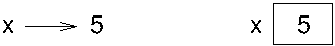
\includegraphics[width=2.5in]{figs/variables.pdf}}
%\caption{Diagrams that represent variables in Python (left) and
%C (right).}
%\label{variables}
%\end{figure}



\section{The compilation process}

As a programmer, you should have a mental model of what happens
during compilation.  If you understand the process, it will help
you interpret error messages, debug your code, and avoid
common pitfalls.

The steps of compilation are:

\begin{enumerate}

\item Preprocessing: C is one of several languages that include
  ``preprocessing directives'' that take effect before the program is
  compiled.  For example, the \verb"#include" directive causes the
  source code from another file to be inserted at the location of the
  directive.

\item Parsing: During parsing, the compiler reads the source code and
  builds an internal representation of the program, called an
  ``abstract syntax tree.''  Errors
  detected during this step are generally syntax errors.

\item Static checking: The compiler checks whether variables and
  values have the right type, whether functions are called with the
  right number and type of arguments, etc.  Errors detected during
  this step are sometimes called ``static semantic'' errors.

\item Code generation: The compiler reads the internal representation
  of the program and generates machine code or byte code.

\item Linking: If the program uses values and functions defined in a
  library, the compiler has to find the appropriate library and
  include the required code.

\item Optimization: At several points in the process, the compiler
  can transform the program to generate code that runs faster or
  uses less space.  Most optimizations are simple changes that eliminate
  obvious waste, but some compilers perform sophisticated analyses and
  transformations.

\end{enumerate}

Normally when you run {\tt gcc}, it runs all of these steps and
generates an executable file.  For example, here is a minimal C
program:

\begin{verbatim}
#include <stdio.h>
int main()
{
    printf("Hello World\n");
}
\end{verbatim}

If you save this code in a file called
{\tt hello.c}, you can compile and run it like this:

\begin{verbatim}
$ gcc hello.c
$ ./a.out
\end{verbatim}

By default, {\tt gcc} stores the executable code in a file
called {\tt a.out} (which originally stood for ``assembler output'').
The second line runs the executable.  The prefix \verb"./" tells
the shell to look for it in the current directory.

It is usually a good idea to use the {\tt -o} flag to provide a
better name for the executable:

\begin{verbatim}
$ gcc hello.c -o hello
$ ./hello
\end{verbatim}


\section{Object code}

The {\tt -c} flag tells {\tt gcc} to compile the program and
generate machine code, but not to link it or generate an executable:

\begin{verbatim}
$ gcc hello.c -c
\end{verbatim}

The result is a file named {\tt hello.o}, where the {\tt o} stands for
``object code'', which is the compiled program.  Object code is not
executable, but it can be linked into an executable.

The UNIX command {\tt nm} reads an object file and generates
information about the names it defines and uses.  For example:

\begin{verbatim}
$ nm hello.o
0000000000000000 T main
                 U puts
\end{verbatim}

This output indicates that {\tt hello.o} defines the name {\tt main}
and uses a function named {\tt puts}, which stands for ``put string.''
In this example, {\tt gcc} performs an optimization by replacing
{\tt printf}, which is a large and complicated function, with
{\tt puts}, which is relatively simple.

You can control how much optimization {\tt gcc} does with
the {\tt -O} flag.  By default, it does very little optimization, which
can make debugging easier.  The option {\tt -O1} turns on the most
common and safe optimizations.  Higher numbers turn on additional
optimizations that require longer compilation time.

In theory, optimization should not change the behavior of the program,
other than to speed it up.  But if your program has a subtle bug,
you might find that optimization makes the bug appear or disappear.
It is usually a good idea to turn off optimization while you are developing
new code.  Once the program is working and passing appropriate tests,
you can turn on optimization and confirm that the tests still pass.


\section{Assembly code}

Similar to the {\tt -c} flag, the {\tt -S} flag tells {\tt gcc}
to compile the program and generate assembly code, which is basically
a human-readable form of machine code.

\begin{verbatim}
$ gcc hello.c -S
\end{verbatim}

The result is a file named {\tt hello.s}, which might look something like
this:

\begin{verbatim}
        .file        "hello.c"
        .section     .rodata
.LC0:
        .string      "Hello World"
        .text
        .globl       main
        .type        main, @function
main:
.LFB0:
        .cfi_startproc
        pushq %rbp
        .cfi_def_cfa_offset 16
        .cfi_offset 6, -16
        movq %rsp, %rbp
        .cfi_def_cfa_register 6
        movl $.LC0, %edi
        call puts
        movl $0, %eax
        popq %rbp
        .cfi_def_cfa 7, 8
        ret
        .cfi_endproc
.LFE0:
        .size        main, .-main
        .ident       "GCC: (Ubuntu/Linaro 4.7.3-1ubuntu1) 4.7.3"
        .section     .note.GNU-stack,"",@progbits
\end{verbatim}

{\tt gcc} is usually configured to generate code for the machine you
are running on, so for me it generates x86 assembly language,
which runs on a wide variety of processors from Intel, AMD, and
others.  If you are running on a different architecture, you might
see different code.


\section{Preprocessing}

Taking another step backward through the compilation process, you
can use the {\tt -E} flag to run the preprocessor only:

\begin{verbatim}
$ gcc hello.c -E
\end{verbatim}

The result is the output from the preprocessor.  In this example,
it contains the included code from {\tt stdio.h}, and all the files
included from {\tt stdio.h}, and all the files included from those
files, and so on.  On my machine, the total is more than 800 lines
of code.  Since almost every C program includes {\tt stdio.h}, those
800 lines of code get compiled a lot.  If, like many C programs,
you also include {\tt stdlib.h}, the result is more than 1800 lines
of code.


\section{Understanding errors}

Now that we know the steps in the compilation process, it is easier
to understand error messages.  For example, if there is an error
in a \verb"#include" directive, you'll get a message from the
preprocessor:

\begin{verbatim}
hello.c:1:20: fatal error: stdioo.h: No such file or directory
compilation terminated.
\end{verbatim}

If there's a syntax error, you get a message from the compiler:

\begin{verbatim}
hello.c: In function 'main':
hello.c:6:1: error: expected ';' before '}' token
\end{verbatim}

If you use a function that's not defined in any of the standard
libraries, you get a message from the linker:

\begin{verbatim}
/tmp/cc7iAUbN.o: In function `main':
hello.c:(.text+0xf): undefined reference to `printff'
collect2: error: ld returned 1 exit status
\end{verbatim}

{\tt ld} is the name of the UNIX linker, so named because ``loading''
is another step in the compilation process that is closely related
to linking.

Once the program starts, C does very little runtime checking,
so there are only a few runtime errors you are likely to see.  If you
divide by zero, or perform another illegal floating-point operation, you
will get a ``Floating point exception.''  And if you try to read or
write an incorrect location in memory, you will get a ``Segmentation
fault.''

% TODO: -Wall and lint


\chapter{Processes}

\section{Abstraction and virtualization}

Before we talk about processes, I want to define a few words:

\begin{itemize}

\item Abstraction: An abstraction is a simplified representation
of something complicated.  For example, if you drive a car, you
understand that when you turn the wheel left, the car goes left,
and vice versa.  Of course, the steering wheel is connected to
a sequence of mechanical and (often) hydraulic systems that turn
the wheels, and the wheels interact with the road in ways that
can be complex, but as a driver, you normally don't have to think
about any of those details.  You can get along very well with
a simple mental model of steering.  Your mental model is an
abstraction.

Similarly, when you use a web browser, you understand that when
you click on a link, the browser displays the page the link refers
to.  The software and network communication that make that possible
are complex, but as a user, you don't have to know the
details.

A large part of software engineering is designing abstractions like
these that allow users and other programmers to use powerful
and complicated systems without having to know about the details
of their implementation.

\item Virtualization: An important kind of abstraction is
virtualization, which is the process of creating a desirable
illusion.

For example, many public libraries participate in inter-library
collaborations that allow them to borrow books from each other.
When I request a book, sometimes the book is on the shelf at my
local library, but other times it has to be transferred from another
collection.  Either way, I get a notification when it is available
for pickup.  I don't need to know where it came from, and I don't
need to know which books my library has.  As a whole, the system
creates the illusion that my library has every book in the world.

The collection physically located at my local library might be small,
but the collection available to me virtually includes every book
in the inter-library collaboration.

As another example, most computers are only connected to one
network, but that network is connected to others, and so on.  What
we call the Internet is a collection of networks and a set of
protocols that forward packets from one network to the next.
From the point of view of a user or programmer, the system behaves
as if every computer on the Internet is connected to every other
computer.  The number of physical connections is small, but the
number of virtual connections is very large.

\end{itemize}

The word ``virtual'' is often used in the context of a virtual
machine, which is software that creates the illusion of a dedicated
computer running a particular operating system, when in reality
the virtual machine might be running, along with many other virtual
machines, on a computer running a different operating system.

In the context of virtualization, we sometimes call what is
really happening ``physical'', and what is virtually happening
either ``logical'' or ``abstract.''


\section{Isolation}

One of the most important principles of engineering is isolation:
when you are designing a system with multiple components, it is usually
a good idea to isolate them from each other so that a change in one
component doesn't have undesired effects on other components.

One of the most important goals of an operating system is to isolate
each running program from the others so that programmers don't have to
think about every possible interaction.  The software object that
provides this isolation is a {\bf process}.

A process is a software object that represents a running program.
I mean ``software object'' in the sense of object-oriented programming;
in general, an object contains data and provides methods
that operate on the data.  A process is an object that contains the
following data:

\begin{itemize}

\item The text of the program, usually a sequence of
  machine language instructions.

\item Data associated with the program, including static data (allocated
  at compile time) and dynamic data including the call stack and
  the heap.

\item The state of any pending input/output operations.  For example,
  if the process is waiting for data to be read from disk or for a
  packet to arrive on a network, the status of these operations is
  part of the process.

\item The hardware state of the program, which includes data stored
  in registers, status information, and the program counter, which
  indicates which instruction is currently executing.

\end{itemize}

Usually one process runs one program, but it is also possible for
a process to load and run a new program.

It is also possible, and common, to run the same program in more than one
process.  In that case, the processes share the same program text,
but generally have different data and hardware states.

Most operating systems provide a fundamental set of capabilities
to isolate processes from each other:

\begin{itemize}

\item Multitasking: Most operating systems have the ability to
  interrupt a running process at almost any time, save its hardware
  state, and then resume the process later.  In general, programmers
  don't have to think about these interruptions.  The program behaves
  as if it is running continuously on a dedicated processor, 
  except that the time between instructions is unpredictable.

\item Virtual memory: Most operating systems create the
  illusion that each process has its own chunk of memory, isolated
  from all other processes.  Again, programmers generally don't
  have to think about how virtual memory works; they can proceed
  as if every program has a dedicated chunk of memory.

\item Device abstraction: Processes running on the same computer share
  the disk drive, the network interface, the graphics card, and other
  hardware.  If processes interacted with this hardware directly,
  without coordination, chaos would ensue.  For example, network data
  intended for one process might be read by another.  Or multiple
  processes might try to store data in the same location on a hard
  drive.  It is up to the operating system to maintain order by
  providing appropriate abstractions.

\end{itemize}

As a programmer, you don't need to know much about how these
capabilities are implemented.  But if you are
curious, you will find a lot of interesting things
going on under the metaphorical hood.  And if you know what's
going on, it can make you a better programmer.


\section{UNIX processes}
\label{unixps}

While I write this book, the process I
am most aware of is my text editor, emacs.  Every once in a while
I switch to a terminal window, which is a window running a UNIX shell
that provides a command-line interface.

When I move the mouse, the window manager wakes up, sees that the
mouse is over the terminal window, and wakes up the terminal.
The terminal wakes up the shell.
If I type {\tt make} in the shell, it creates a
new process to run Make, which creates another process to run LaTeX
and then another process to display the results.

If I need to look something up, I might switch to another desktop,
which wakes up the window manager again.  If I click on the icon for a
web browser, the window manager creates a process to run the web
browser.  Some browsers, like Chrome, create a new process for each
window and each tab.

And those are just the processes I am aware of.  At the same time
there are many other processes running ``in the background.''
Many of them are performing operations related to the operating
system.

The UNIX command {\tt ps} prints information about running processes.
If you run it in a terminal, you might see something like this:

\begin{verbatim}
  PID TTY          TIME CMD
 2687 pts/1    00:00:00 bash
 2801 pts/1    00:01:24 emacs
24762 pts/1    00:00:00 ps
\end{verbatim}

The first column is the unique numerical process ID.  The second
column is the terminal that created the process; 
``TTY'' stands for teletypewriter, which was the original
mechanical terminal.

The third column is the total processor time used by the process,
in hours, minutes, and seconds.
The last column is the name of the running program.  In
this example, {\tt bash} is the name of the shell that interprets
the commands I type in the terminal, emacs is my text editor, and
ps is the program generating this output.

By default, {\tt ps} lists only the processes associated with
the current terminal.  If you use the {\tt -e} flag, you get every
process (including processes belonging to other users, which is
a security flaw, in my opinion).

On my system there are currently 233 processes.
Here are some of them:

\begin{verbatim}
  PID TTY          TIME CMD
    1 ?        00:00:17 init
    2 ?        00:00:00 kthreadd
    3 ?        00:00:02 ksoftirqd/0
    4 ?        00:00:00 kworker/0:0
    8 ?        00:00:00 migration/0
    9 ?        00:00:00 rcu_bh
   10 ?        00:00:16 rcu_sched
   47 ?        00:00:00 cpuset
   48 ?        00:00:00 khelper
   49 ?        00:00:00 kdevtmpfs
   50 ?        00:00:00 netns
   51 ?        00:00:00 bdi-default
   52 ?        00:00:00 kintegrityd
   53 ?        00:00:00 kblockd
   54 ?        00:00:00 ata_sff
   55 ?        00:00:00 khubd
   56 ?        00:00:00 md
   57 ?        00:00:00 devfreq_wq
\end{verbatim}

{\tt init} is the first process created when the operating system
starts.  It creates many of the other processes, and then sits idle
until the processes it created are done.

{\tt kthreadd} is a process the operating system uses to create new
``threads''.  We'll talk more about threads later, but for now you can
think of a thread as kind of a process.  The {\tt k} at the beginning
stands for ``kernel'' which is the part of the operating system
responsible for core capabilities like creating threads.  The extra
{\tt d} at the end stands for ``daemon'', which is another name for
processes like this that run in the background and provide operating
system services.  In this context, ``daemon'' is used in the
sense of a helpful spirit, with no connotation of evil.

Based on the name, you can infer that {\tt ksoftirqd} is also a kernel
daemon; specifically, it handles software interrupt requests, or
``soft IRQ''.

{\tt kworker} is a worker process created by the kernel to do some
kind of processing for the kernel.

There are often multiple processes running these kernel services.
On my system at the moment, there are 8 {\tt ksoftirqd} processes
and 35 {\tt kworker} processes.

I won't go into more details about the other processes, but if you
are interested you can search for more information about them.
You should run {\tt ps} on your system and compare your results
to mine.

%TODO: using gdb here?


\chapter{Virtual memory}

\section{A bit of information theory}

A bit is a binary digit; it is also a unit of information.  If you
have one bit, you can specify one of two possibilities, usually
written 0 and 1.  If you have two bits, there are 4 possible
combinations, 00, 01, 10, and 11.  In general, if you have $b$ bits, you
can indicate one of $2^b$ values.  A byte is 8 bits, so it can
hold one of 256 values.

Going in the other direction, suppose you want to store a letter
of the alphabet.  There are 26 letters, so how many bits do you
need?  With 4 bits, you can specify one of 16 values, so that's
not enough.  With 5 bits, you can specify up to 32 values, so
that's enough for all the letters, with a few values left over.

In general, if you want to specify one of $N$ values, you should
choose the smallest value of $b$ so that $2^b \ge N$.  Taking the
log base 2 of both sides yields $b \ge log_2 N$.

Suppose I flip a coin and tell you the outcome.  I have given
you one bit of information.  If I roll a six-sided die and tell
you the outcome, I have given you $log_2 6$ bits of information.
And in general, if the probability of the outcome is 1 in $N$,
then the outcome contains $log_2 N$ bits of information.

Equivalently, if the probability of the outcome is $p$, then
the information content is $-log_2 p$.  This quantity is called
the ``self-information'' of the outcome.  It measures
how surprising the outcome is, which is why it is also called
``surprisal.''  If your horse has only one chance in 16 of winning,
and he wins, you get 4 bits of information (along with the
payout).  But if the favorite wins 75\% of the time, the news
of the win contains only 0.42 bits.

Intuitively, unexpected news carries a lot of
information; conversely, if there is something you were already confident
of, confirming it contributes only a small amount of information.

For several topics in this book, we will need to be comfortable
converting back and forth between the number of bits, $b$, and the
number of values they can encode, $N = 2^b$.


\section{Memory and storage}

While a process is running, most of its data is held in ``main
memory'', which is usually some kind of random access memory (RAM).
On most current computers, main memory is volatile, which means that
when the computer shuts down, the contents of main memory are lost.
A typical desktop computer has 2--8 GiB of
memory.  GiB stands for ``gibibyte,'' which is $2^{30}$ bytes.  

If the process reads and writes files, those files are usually stored
on a hard disk drive (HDD) or solid state drive (SSD).  These storage
devices are non-volatile, so they are used for long-term storage.
Currently a typical desktop computer has a HDD with a capacity of 500
GB to 2 TB.  GB stands for ``gigabyte,'' which is $10^9$ bytes.  TB
stands for ``terabyte,'' which is $10^{12}$ bytes.

You might have noticed that I used the binary unit
GiB for the size of main memory and the decimal units GB and TB for
the size of the HDD.  For historical and technical reasons, memory is
measured in binary units, and disk drives are measured in decimal
units.  In this book I will be careful to distinguish binary and
decimal units, but you should be aware that the word ``gigabyte'' and the
abbreviation GB are often used ambiguously.

In casual use, the term ``memory'' is sometimes used for HDDs and SSDs
as well as RAM, but the properties of these devices are very
different, so we will need to distinguish them.  I will use
``storage'' to refer to HDDs and SSDs.


\section{Address spaces}

Each byte in main memory is specified by an integer ``physical
address''.  The set of valid physical addresses is called the
physical ``address space.''  It
usually runs from 0 to $N-1$, where $N$ is
the size of main memory.  On a system with 1 GiB of physical memory,
the highest valid address is $2^{30}-1$, which is 1,073,741,823 in
decimal, or 0x03ff ffff in hexadecimal (the prefix 0x indicates a
hexadecimal number).

However, most operating systems provide ``virtual memory,'' which
means that programs never deal with physical addresses, and don't 
have to know how much physical memory is available.

Instead, programs work with virtual addresses, which are numbered
from 0 to $M-1$, where $M$ is the number of valid virtual addresses.
The size of the virtual address space is determined by the operating
system and the hardware it runs on.

You have probably heard people talk about 32-bit and 64-bit systems.
These terms indicate the size of the registers, which is usually also
the size of a virtual address.  On a 32-bit system, virtual addresses
are 32 bits, which means that the virtual address space runs from 0 to
0xffff ffff.  The size of this address space is $2^{32}$ bytes, or 4
GiB.

On a 64-bit system, the size of the virtual address space is $2^{64}$
bytes, or $4 \cdot 1024^6$ bytes.  That's 16 exbibytes, which is
about a billion times bigger than current physical memories.  It might
seem strange that a virtual address space can be so much bigger
than physical memory, but we will see soon how that works.

When a program reads and writes values in memory, it generates virtual
addresses.  The hardware, with help from the operating system,
translates to physical addresses before accessing main memory.  This
translation is done on a per-process basis, so even if two processes
generate the same virtual address, they would map to different
locations in physical memory.

Thus, virtual memory is one important way the operating system
isolates processes from each other.  In general, a process cannot
access data belonging to another process, because there is no
virtual address it can generate that maps to physical memory
allocated to another process.



\section{Memory segments}

The data of a running process is organized into five segments:

\begin{itemize}

\item The code segment contains the program text; that is, the
  machine language instructions that make up the program.

\item The static segment contains immutable values, like string
literals.  For example, if your program contains the string
{\tt "Hello, World"}, those characters will be stored in the
static segment.

\item The globals segment contains global variables and local variables that are declared {\tt static}.

\item The heap segment contains chunks of memory allocated
  at run time, usually by calling the C library function
  {\tt malloc}.

\item The stack segment contains the call stack, which is a
  sequence of stack frames.  Each time a function is called, a stack
  frame is allocated to contain the 
  parameters and local variables of the function.  When the function
  completes, its stack frame is removed from the stack.

\end{itemize}

The arrangement of these segments is determined partly by the 
compiler and partly by the operating system.  The details vary
from one system to another, but in the most common arrangement:

\begin{itemize}

\item The text segment is near the ``bottom'' of memory, that is,
  at addresses near 0.

\item The static segment is often just above the text segment, that is,
at higher addresses.

\item The global segment is often just above the static segment.

\item The heap is often above the global segment.  As it expands,
  it grows up toward larger addresses.
  
\item The stack is near the top of memory; that is, near the
  highest addresses in the virtual address space.  As the
  stack expands, it grows down toward smaller addresses.

\end{itemize}

%TODO: Figure out how to handle the code that is in both ExercisesInC
% and the repo for the book.

To determine the layout of these segments on your system, try running
this program, which is in {\tt aspace.c} in the repository for this
book (see Section~\ref{code}).

\begin{verbatim}
#include <stdio.h>
#include <stdlib.h>

int global;

int main ()
{
    int local = 5;
    void *p = malloc(128);
    char *s = "Hello, World";

    printf ("Address of main is %p\n", main);
    printf ("Address of global is %p\n", &global);
    printf ("Address of local is %p\n", &local);
    printf ("p points to %p\n", p);
    printf ("s points to %p\n", s);
}
\end{verbatim}

{\tt main} is the name of a function; when it is used as a variable,
it refers to the address of the first machine language instruction
in {\tt main}, which we expect to be in the text segment.

{\tt global} is a global variable, so we expect it to be in the
global segment.  {\tt local} is a local variable, so we expect it
to be on the stack.

{\tt s} refers to a ``string literal", which is a string that appears
as part of the program (as opposed to a string that is read from a file,
input by a user, etc.).  We expect the location of the string to be
in the static segment (as opposed to the pointer, {\tt s}, which is
a local variable).

{\tt p} contains an address returned by {\tt malloc}, which allocates
space in the heap.  ``malloc'' stands for ``memory allocate.''

The format sequence \verb"%p" tells {\tt printf} to format each
address as a ``pointer'', so it displays the results in hexadecimal.

When I run this program, the output looks like this (I added spaces
to make it easier to read):

\begin{verbatim}
Address of main is   0x      40057d
Address of global is 0x      60104c
Address of local is  0x7ffe6085443c
p points to          0x     16c3010
s points to          0x      4006a4

\end{verbatim}

As expected, the address of {\tt main} is the lowest, followed by
the location of the string literal.  The location of
{\tt global} is next, then the address {\tt p} points to.
The address of {\tt local} is much bigger.

The largest address has 12 hexadecimal digits.  Each hex digit
corresponds to 4 bits, so it is a 48-bit address.  That suggests
that the usable part of the virtual address space is $2^{48}$ bytes.

As an exercise, run this program on your computer and compare your
results to mine.  Add a second call to {\tt malloc} and check whether
the heap on your system grows up (toward larger addresses).  Add a
function that prints the address of a local variable, and check
whether the stack grows down.


\section{Static local variables}

Local variables on the stack are sometimes called ``automatic'',
because they are allocated automatically when a function is called,
and freed automatically when the function returns.

In C there is another kind of local variable, called ``static'',
which is allocated in the global segment.  It is initialized when
the program starts and keeps its value from one function call to
the next.

For example, the following function keeps track of how many times
it has been called.

\begin{verbatim}
int times_called()
{
    static int counter = 0;
    counter++;
    return counter;
}
\end{verbatim}

The keyword {\tt static} indicates that {\tt counter} is a static
local variable.  The initialization happens only once, when the program
starts.

If you add this function to {\tt aspace.c} you can confirm that
{\tt counter} is allocated in the static segment along with global
variables, not in the stack.


\section{Address translation}
\label{address_translation}

How does a virtual address (VA) get translated to a physical address
(PA)?  The basic mechanism is simple, but a simple
implementation would be too slow and take too much space.  So actual
implementations are a bit more complicated.

Most processors provide a memory management unit (MMU) that
sits between the CPU and main memory.  The MMU performs fast
translation between VAs and PAs.

\begin{enumerate}

\item When a program reads or writes a variable, the CPU generates a
VA.  

\item The MMU splits the VA into two parts, called the page number and
the offset.  A ``page'' is a chunk of memory; the size of a page
depends on the operating system and the hardware, but common sizes
are 1--4 KiB.

\item The MMU looks up the page number in the translation lookaside buffer (TLB) and gets the corresponding physical page number.  Then it combines
the physical page number with the offset to produce a PA.

\item The PA is passed to main memory, which reads or writes the given
location.

\end{enumerate}

The TLB contains cached copies of data from the page table (which is stored in kernel memory).  The page table contains the mapping from virtual page numbers to physical page numbers.  Since each process has its own page table, the TLB has to make sure it only uses entries from the page table of the process that's running.

To see how all this works, suppose that the VA is 32 bits and the physical memory is 1 GiB, divided into 1 KiB pages.

\begin{itemize}

\item Since 1 GiB is $2^{30}$ bytes and 1 KiB is $2^{10}$ bytes, there
  are $2^{20}$ physical pages, sometimes called ``frames.''

\item The size of the virtual address space is $2^{32}$ B and the size
  of a page is $2^{10}$ B, so there are $2^{22}$ virtual pages.

\item The size of the offset is determined by the page size.  In this
  example the page size is $2^{10}$ B, so it takes 10 bits to specify
  a byte on a page.

\item If a VA is 32 bits and the offset is 10 bits, the remaining
  22 bits make up the virtual page number.

\item Since there are $2^{20}$ physical pages, each physical page
  number is 20 bits.  Adding in the 10 bit offset, the resulting
  PAs are 30 bits.

\end{itemize}

So far this all seems feasible.  But let's think about how big a page
table might have to be.  The simplest implementation of a page
table is an array with one entry for each virtual page.
Each entry would contain a physical page number, which is 20 bits
in this example, plus some additional information about each
frame.  So we expect 3--4 bytes per entry.  But with $2^{22}$ virtual pages,
the page table would require $2^{24}$ bytes, or 16 MiB.

And since we need a page table for each process, a system running
256 processes would need $2^{32}$ bytes, or 4 GiB, just for page tables!
And that's just with 32-bit virtual addresses.  With 48- or 64-bit
VAs, the numbers are ridiculous.

Fortunately, we don't actually need that much space, because
most processes don't use even a small fraction of their
virtual address space.  And if a process doesn't use a virtual
page, we don't need an entry in the page table for it.

Another way to say the same thing is that page tables are ``sparse'',
which implies that the simple implementation, an array of page
table entries, is a bad idea.  Fortunately, there are several
good implementations for sparse arrays.

One option is a multilevel page table, which is what many operating
systems, including Linux, use.  Another option is an associative table, where each entry includes both the virtual page number and the physical page number.  Searching an associative table can be slow in software, but in hardware we
can search the entire table in parallel, so associative arrays are
often used to represent the page table entries in the TLB.

You can read more about these implementations at
\url{http://en.wikipedia.org/wiki/Page_table}; you might find the
details interesting.  But the fundamental idea is that page tables are
sparse, so we have to choose a good implementation for sparse arrays.

I mentioned earlier that the operating system can interrupt a running
process, save its state, and then run another process.  This mechanism
is called a ``context switch''.  Since each process has its own
page table, the operating system has to work with the MMU to make
sure each process gets the right page table.  In older machines,
the page table information in the MMU had to be replaced during every
context switch, which was expensive.  In newer systems, each page
table entry in the MMU includes the process ID, so page tables from
multiple processes can be in the MMU at the same time.



\chapter{Files and file systems}

When a process completes (or crashes), any data stored in main
memory is lost.  But data stored on a hard disk drive (HDD) or
solid state drive (SSD) is ``persistent;'' that is, it survives
after the process completes, even if the computer shuts down.

Hard disk drives are complicated.  Data is stored in blocks, which
are laid out in sectors, which make up tracks, which are arranged
in concentric circles on platters.

Solid state drives are simpler in one sense, because blocks are
numbered sequentially, but they raise a different complication: each
block can be written a limited number of times before it becomes
unreliable.

As a programmer, you don't want to deal with these complications.
What you want is an appropriate abstraction of persistent storage
hardware.  The most common abstraction is called a ``file system.''

Abstractly:

\begin{itemize}

\item A ``file system'' is a mapping from each file's name to its contents.
If you think of the names as keys, and the contents as values,
a file system is a kind of key-value database
(see \url{https://en.wikipedia.org/wiki/Key-value_database}).

\item A ``file'' is a sequence of bytes.

\end{itemize}

File names are usually strings, and they are usually ``hierarchical'';
that is, the string specifies a path from a top-level directory (or
folder), through a series of subdirectories, to a specific file.

The primary difference between the abstraction and the underlying
mechanism is that files are byte-based and persistent storage is
block-based.  The operating system translates byte-based file operations 
in the C library into block-based operations on storage devices.
Typical block sizes are 1--8 KiB.

For example, the following code opens a file and reads the first byte:

\begin{verbatim}
    FILE *fp = fopen("/home/downey/file.txt", "r");
    char c = fgetc(fp);
    fclose(fp);
\end{verbatim}

When this code runs:

\begin{enumerate}

\item {\tt fopen} uses the filename to find the top-level directory,
  called \verb"/", the subdirectory {\tt home}, and the
  sub-subdirectory {\tt downey}.

\item It finds the file named {\tt file.txt} and ``opens'' it for
  reading, which means it creates a data structure that represents the
  file being read.  Among other things, this data structure
  keeps track of how much of the file has been read, called the ``file
  position''.

  In DOS, this data structure is called a File Control Block, but I
  want to avoid that term because in UNIX it means something else.  In
  UNIX, there seems to be no good name for it.  It is an entry in the
  open file table, so I will call it an OpenFileTableEntry.

\item When we call {\tt fgetc}, the operating system checks whether
  the next character of the file is already in memory.  If so, it
  reads the next character, advances the file position, and returns
  the result.

\item If the next character is not in memory, the operating
  system issues an I/O request to get the next block.  Disk drives are
  slow, so a process waiting for a block from disk is usually
  interrupted so another process can run until the data arrives.

\item When the I/O operation is complete, the new block of data is
  stored in memory, and the process resumes.  It reads the first
  character and stores it as a local variable.

\item When the process closes the file, the operating system completes
  or cancels any pending operations, removes data stored in
  memory, and frees the OpenFileTableEntry.

\end{enumerate}

The process for writing a file is similar, but there are some
additional steps.  Here is an example that opens a file for
writing and changes the first character.

\begin{verbatim}
    FILE *fp = fopen("/home/downey/file.txt", "w");
    fputc('b', fp);
    fclose(fp);
\end{verbatim}

When this code runs:

\begin{enumerate}

\item Again, {\tt fopen} uses the filename to find the file.  If it
  does not already exist, it creates a new file and adds an entry in
  the parent directory, {\tt /home/downey}.

\item The operating system creates an OpenFileTableEntry that
  indicates that the file is open for writing, and sets the file
  position to 0.

\item {\tt fputc} attempts to write (or re-write) the first byte of
  the file.  If the file already exists, the operating system has to
  load the first block into memory.  Otherwise it allocates a new
  block in memory and requests a new block on disk.

\item After the block in memory is modified, it might not be copied
  back to the disk right away.  In general, data written to a file is
  ``buffered'', which means it is stored in memory and only written to
  disk when there is at least one block to write.

\item When the file is closed, any buffered data is written to disk
  and the OpenFileTableEntry is freed.

\end{enumerate}

To summarize, the C library provides the abstraction of a file
system that maps from file names to streams of bytes.  This abstraction
is built on top of storage devices that are actually organized
in blocks.


\section{Disk performance}

\newcommand{\mus}{$\mu$s~}

I mentioned earlier that disk drives are slow.  On current HDDs, the
average time to read a block from disk to memory might be 5--25 ms
(see \url{https://en.wikipedia.org/wiki/Hard_disk_drive_performance_characteristics}).
SSDs are faster, taking 25 \mus to read a 4 KiB block and 250 \mus to
write one (see \url{http://en.wikipedia.org/wiki/Ssd#Controller}).

To put these numbers in perspective, let's compare them to the clock
cycle of the CPU.  A processor with clock rate 2 GHz completes one
clock cycle every 0.5 ns.  The time to get a byte from memory to
the CPU is typically around 100 ns.  If the processor completes one
instruction per clock cycle, it would complete 200 instructions
while waiting for a byte from memory.

In one microsecond, it would complete 2000 instructions,
so while waiting 25 \mus for a byte from an SSD, it would complete 50,000.

In one millisecond, it would complete 2,000,000 instructions,
so while waiting 20 ms for a byte from a HDD, it might complete
40 million.  If there's nothing for the CPU to do while it waits,
it would be idle.  That's why the operating system generally
switches to another process while it is waiting for data from disk.

The gap in performance between main memory and persistent storage is
one of the major challenges of computer system design.  Operating
systems and hardware provide several features intended to ``fill in''
this gap:

\begin{itemize}

\item Block transfers: The time it takes to load a single byte from
  disk is 5--25 ms.  By comparison, the additional time to load an 8
  KiB block is negligible.  So systems generally try to read large
  blocks each time they access the disk.

\item Prefetching: Sometimes the operating system can predict that a
  process will read a block and start loading it before it is
  requested.  For example, if you open a file and read the first
  block, there is a good chance you will go on to read the second
  block.  The operating system might start loading additional blocks
  before they are requested.

\item Buffering: As I mentioned, when you write a file, the operating
  system stores the data in memory and only writes it to disk later.
  If you modify the block several times while it is in memory, the
  system only has to write it to disk once.

\item Caching: If a process has used a block recently, it is likely to
  use it again soon.  If the operating system keeps a copy of the
  block in memory, it can handle future requests at memory speed.

\end{itemize}

Some of these features are also implemented in hardware.  For example,
some disk drives provide a cache that stores recently-used blocks,
and many disk drives read more than one block at a time, even if only
one is requested.

These mechanisms generally improve the performance of
programs, but they don't change the behavior.  Usually programmers
don't have to think about them, with two exceptions: (1) if the
performance of a program is unexpectedly bad, you might have to know
something about these mechanisms to diagnose the problem, and (2)
when data is buffered, it can be harder to debug a program.  For
example, if a program prints a value and then crashes, the value
might not appear, because it might be in a buffer.  Similarly, if a
program writes data to disk and then the computer loses power, the
data might be lost if it is in a cache and not yet on disk.


\section{Disk metadata}

The blocks that make up a file might be arranged contiguously on
disk, and file system performance is generally better if they are,
but most operating systems don't require contiguous allocation.
They are free to place a block anywhere on disk, and they use
various data structures to keep track of them.

In many UNIX file systems, that data structure is called an ``inode,''
which stands for ``index node''.  More generally, information about
files, including the location of their blocks, is called ``metadata''.
(The content of the file is data, so information about the file is
data about data, hence ``meta''.)

Since inodes reside on disk along with the rest of the data, they are
designed to fit neatly into disk blocks.  A UNIX inode contains
information about a file, including the user ID of the file owner;
permission flags indicating who is allowed to read, write, or execute
it; and timestamps that indicate when it was last modified and
accessed.  In addition, it contains block numbers for the first 12
blocks that make up the file.

If the block size is 8 KiB, the first 12 blocks make up 96 KiB.
On most systems, that's big enough for a large majority of files,
but it's definitely not big enough for all of them.  That's
why the inode also contains a pointer to an ``indirection block'',
which contains nothing but pointers to other blocks.

The number of pointers in an indirection block depends on the sizes of
the blocks and the block numbers, but it is often 1024.  With 1024
block numbers and 8 KiB blocks, an indirection block can address 8
MiB.  That's big enough for all but the largest files, but still not
big enough for all.

That's why the inode also contains a pointer to a ``double indirection
block'', which contains pointers to indirection blocks.  With
1024 indirection blocks, we can address 8 GiB.

And if that's not big enough, there is (finally) a triple indirection
block, which contains pointers to double indirection blocks, yielding
a maximum file size of 8 TiB.  When UNIX inodes were designed, that
seemed big enough to serve for a long time.  But that was a long time
ago.

As an alternative to indirection blocks, some files systems, like FAT,
use a File Allocation Table that contains one entry for each block,
called a ``cluster'' in this context.  A root directory contains a
pointer to the first cluster in each file.  The FAT entry for each
cluster points to the next cluster in the file, similar to a linked
list.  For more details, see
\url{http://en.wikipedia.org/wiki/File_Allocation_Table}.


\section{Block allocation}

File systems have to keep track of which blocks belong to each file;
they also have to keep track of which blocks are available for use.
When a new file is created, the file system finds an available
block and allocates it.  When a file is deleted, the file system
makes its blocks available for re-allocation.

The goals of the block allocation system are:

\begin{itemize}

\item Speed: Allocating and freeing blocks should be fast.

\item Minimal space overhead: The data structures used by the allocator
  should be small, leaving as much space as possible for data.

\item Minimal fragmentation: If some blocks are left unused, or some
  are only partially used, the unused space is called
  ``fragmentation''.

\item Maximum contiguity: Data that is likely to be used at the same
  time should be physically contiguous, if possible, to improve
  performance.

\end{itemize}

It is hard to design a file system that achieves all of these
goals, especially since file system performance depends on
``workload characteristics'' like file sizes, access
patterns, etc.  A file system that is well tuned for one workload
might not perform as well for another.

For this reason, most operating systems support several kinds of file
systems, and file system design is an active area of research and
development.  In the last decade, Linux systems have migrated
from ext2, which was a conventional UNIX file system, to ext3,
a ``journaling'' file system intended to improve speed and
contiguity, and more recently to ext4, which can handle larger files
and file systems.  Within the next few years, there might be
another migration to the B-tree file system, Btrfs.


\section{Everything is a file?}

The file abstraction is really a ``stream of bytes'' abstraction,
which turns out to be useful for many things, not just file systems.

One example is the UNIX pipe, which is a simple form of inter-process
communication.  Processes can be set up so that output from one
process is taken as input into another process.  For the first
process, the pipe behaves like a file open for writing, so it
can use C library functions like {\tt fputs} and {\tt fprintf}.
For the second process, the pipe behaves like a file open for
reading, so it uses {\tt fgets} and {\tt fscanf}.

Network communication also uses the stream of bytes abstraction.
A UNIX socket is a data structure that represents a communication
channel between processes on different computers (usually).  Again,
processes can read data from and write data to a socket using
``file'' handling functions.

Reusing the file abstraction makes life easier for programmers, since
they only have to learn one API (application program interface).
It also makes programs more versatile, since a program intended to
work with files can also work with data coming from pipes and other
sources.

% TODO: gprof here?


\chapter{More bits and bytes}

\section{Representing integers}

You probably know that computers represent numbers in
base 2, also known as binary.  For positive numbers, the binary
representation is straightforward; for example, the representation
for $5_{10}$ is $b101$.

For negative numbers, the most obvious representation uses
a sign bit to indicate whether a number is positive or negative.
But there is another representation, called ``two's complement''
that is much more common because it is easier to work with
in hardware.

To find the two's complement of a negative number, $-x$, find
the binary representation of $x$, flip all the bits, and add 1.
For example, to represent $-5_{10}$, start with the representation
of $5_{10}$, which is $b0000 0101$ if we write the 8-bit version.
Flipping all the bits and adding 1 yields $b1111 1011$.

In two's complement, the leftmost bit acts like a sign bit;
it is 0 for positive numbers and 1 for negative numbers.

To convert from an 8-bit number to 16-bits, we have to add
more 0's for a positive number and add 1's for a negative number.
In effect, we have to copy the sign bit into the new bits.
This process is called ``sign extension''.

In C all integer types are signed (able to represent positive and
negative numbers) unless you declare them {\tt unsigned}.  The
difference, and the reason this declaration is important, is that
operations on unsigned integers don't use sign extension.


\section{Bitwise operators}

People learning C are sometimes confused
about the bitwise operators \verb"&" and \verb"|".  These
operators treat integers as bit vectors and compute logical
operations on corresponding bits.

For example, \verb"&" computes the AND operation, which yields
1 if both operands are 1, and 0 otherwise.  Here is an example
of \verb"&" applied to two 4-bit numbers:
%
\begin{verbatim}
  1100
& 1010
  ----
  1000
\end{verbatim}
%
In C, this means that the expression \verb"12 & 10" has the
value 8.

Similarly, \verb"|" computes the OR operation, which yields
1 if either operand is 1, and 0 otherwise.
%
\begin{verbatim}
  1100
| 1010
  ----
  1110
\end{verbatim}
%
So the expression \verb"12 | 10" has the value 14.

Finally, \verb"^" computes the XOR operation, which yields
1 if either operand is 1, but not both.
%
\begin{verbatim}
  1100
^ 1010
  ----
  0110
\end{verbatim}
%
So the expression \verb"12 ^ 10" has the value 6.

Most commonly, \verb"&" is used to clear a set of bits from
a bit vector, \verb"|" is used to set bits, and \verb"^"
is used to flip, or ``toggle'' bits.  Here are the details:

{\bf Clearing bits}: For any value $x$, $x \& 0$ is 0, and $x \& 1$ is $x$.
So if you AND a vector with 3, it 
selects only the two rightmost bits, and sets the rest to 0.
%
\begin{verbatim}
  xxxx
& 0011
  ----
  00xx
\end{verbatim}
%
In this context, the value 3 is called a ``mask'' because it
selects some bits and masks the rest.

{\bf Setting bits}: Similarly, for any $x$, $x | 0$ is x, and $x | 1$ is $1$.
So if you OR a vector with 3, it sets the rightmost
bits, and leaves the rest alone:
%
\begin{verbatim}
  xxxx
| 0011
  ----
  xx11
\end{verbatim}
%
{\bf Toggling bits}: Finally, if you XOR a vector with 3, it flips the
rightmost bits and leaves the rest alone.  As an exercise, see if you
can compute the two's complement of 12 using \verb"^".  Hint: what's
the two's complement representation of -1?

% (12 ^ -1) + 1

C also provides shift operators, {\tt <<} and {\tt >>}, which shift
bits left and right.  Each left shift doubles a number, so
{\tt 5 << 1} is 10, and {\tt 5 << 2} is 20.  Each right shift
divides by two (rounding down), so {\tt 5 >> 1} is 2 and
{\tt 2 >> 1} is 1.


\section{Representing floating-point numbers}

Floating-point numbers are represented using the binary
version of scientific notation.  In decimal notation, large
numbers are written as the product of a coefficient and 10 raised
to an exponent.  For example, the speed of light in m/s is
approximately $2.998 \cdot 10^8$.

Most computers use the IEEE standard for floating-point
arithmetic.  The C type {\tt float} usually corresponds
to the 32-bit IEEE standard; {\tt double} usually corresponds
to the 64-bit standard.

In the 32-bit standard, the leftmost bit is the sign bit, $s$.
The next 8 bits are the exponent, $q$, and the last 23 bits are
the coefficient, $c$.  The value of a floating-point number is
%
\[ (-1)^s c \cdot 2^q \]
%
Well, that's almost correct, but there's one more wrinkle.
Floating-point numbers are usually normalized so that there is
one digit before the point.  For example, in base 10, we prefer
$2.998 \cdot 10^8$ rather than $2998 \cdot 10^5$ or any other
equivalent expression.  In base 2, a normalized number always
has the digit 1 before the binary point.  Since the digit in
this location is always 1, we can save space by leaving it
out of the representation.

For example, the integer representation of $13_{10}$ is $b1101$.
In floating point, that's $1.101 \cdot 2^3$, so the exponent
is 3 and the part of the coefficient that would be stored
is 101 (followed by 20 zeros).

Well, that's almost correct, but there's one more wrinkle.
The exponent is stored with a ``bias''.  In the 32-bit standard,
the bias is 127, so the exponent 3 would be stored as 130.

To pack and unpack floating-point numbers in C, we can use a 
union and bitwise operations.  Here's an example:
%
\begin{verbatim}
    union {
        float f;
        unsigned int u;
    } p;

    p.f = -13.0;
    unsigned int sign = (p.u >> 31) & 1;
    unsigned int exp = (p.u >> 23) & 0xff;

    unsigned int coef_mask = (1 << 23) - 1;
    unsigned int coef = p.u & coef_mask;

    printf("%d\n", sign);
    printf("%d\n", exp);
    printf("0x%x\n", coef);
\end{verbatim}
%
This code is in {\tt float.c} in the repository for this
book (see Section~\ref{code}).

The union allows us to store a floating-point value using
{\tt p.f} and then read it as an unsigned integer using
{\tt p.u}.

To get the sign bit, we shift the bits to the right 31
places and then use a 1-bit mask to select only the
rightmost bit.

To get the exponent, we shift the bits 23 places, then select the
rightmost 8 bits (the hexadecimal value {\tt 0xff} has eight 1's).

To get the coefficient, we need to extract the 23 rightmost bits
and ignore the rest.  We do that by making a mask with 1s in the
23 rightmost places and 0s on the left.  The easiest way to do that
is by shifting 1 to the left by 23 places and then subtracting 1.  

The output of this program is:
%
\begin{verbatim}
1
130
0x500000
\end{verbatim}
%
As expected, the sign bit for a negative number is 1.  The exponent 
is 130, including the bias.  And the coefficient, which I printed in
hexadecimal, is $101$ followed by 20 zeros.

As an exercise, try assembling or disassembling a {\tt double}, which
uses the 64-bit standard.  See
\url{http://en.wikipedia.org/wiki/IEEE_floating_point}.


\section{Unions and memory errors}

There are two common uses of C unions.  One, which we saw in the
previous section, is to access the binary representation of data.
Another is to store heterogeneous data.  For example, you could
use a union to represent a number that might be an integer, float,
complex, or rational number.

However, unions are error-prone.  It is up to you, as the programmer,
to keep track of what type of data is in the union; if you write
a floating-point value and then interpret it as an integer, the result
is usually nonsense.

Actually, the same thing can happen if you read a location in memory
incorrectly.  One way that can happen is if you read past the end of
an array.

To see what happens, I'll start with a function that allocates an
array on the stack and fills it with the numbers from 0 to 99.

\begin{verbatim}
void f1() {
    int i;
    int array[100];

    for (i=0; i<100; i++) {
        array[i] = i;
    }
}
\end{verbatim}

Next I'll define a function that creates a smaller array and
deliberately accesses elements before the beginning and after
the end:

\begin{verbatim}
void f2() {
    int x = 17;
    int array[10];
    int y = 123;

    printf("%d\n", array[-2]);
    printf("%d\n", array[-1]);
    printf("%d\n", array[10]);
    printf("%d\n", array[11]);
}
\end{verbatim}

If I call {\tt f1} and then {\tt f2}, I get these results:

\begin{verbatim}
17
123
98
99
\end{verbatim}

The details here depend on the compiler, which arranges variables
on the stack.  From these results, we can infer that the
compiler put {\tt x} and {\tt y} next to each other, ``below''
the array (at a lower address).  And when we read past the
array, it looks like we are getting values that were left on
the stack by the previous function call.

In this example, all of the variables are integers, so it is
relatively easy to figure out what is going on.  But in general
when you read beyond the bounds of an array, the values you
read might have any type.  For example, if I change {\tt f1}
to make an array of floats, the results are:

\begin{verbatim}
17
123
1120141312
1120272384
\end{verbatim}

The latter two values are what you get if you interpret a
floating-point value as an integer.  If you encountered this output
while debugging, you would have a hard time figuring out what's
going on.


\section{Representing strings}

Related issues sometimes come up with strings.  First, remember
that C strings are null-terminated.  When you allocate space
for a string, don't forget the extra byte at the end.

Also, the letters {\it and numbers} in C strings are
encoded in ASCII.  The ASCII codes for the digits ``0'' through ``9''
are 48 through 57, {\it not} 0 through 9.  The ASCII code 0 is the NUL
character that marks the end of a string.  And the ASCII codes 1
through 9 are special characters used in some communication protocols.
ASCII code 7 is a bell; on some terminals, printing it makes a sound.

The ASCII code for the letter ``A'' is 65; the code for
``a'' is 97.  Here are those codes in binary:

\begin{verbatim}
65 = b0100 0001
97 = b0110 0001
\end{verbatim}

A careful observer will notice that they differ by a single
bit.  And this pattern holds for the rest of the letters; the
sixth bit (counting from the right) acts as a ``case bit'', 0 for
upper-case letters and 1 for lower case letters.

As an exercise, write a function that takes a string and converts
from lower-case to upper-case by flipping the sixth bit.  As a challenge,
you can make a faster version by reading the string 32 or 64 bits
at a time, rather than one character at a time.  This optimization
is made easier if the length of the string is a multiple of 4 or
8 bytes.

If you read past the end of a string, you are likely to see
strange characters.  Conversely, if you write a string and
then accidentally read it as an int or float, the results
will be hard to interpret.

For example, if you run:

\begin{verbatim}
    char array[] = "allen";
    float *p = array;
    printf("%f\n", *p);
\end{verbatim}

You will find that the ASCII representation of the first 8 characters
of my name, interpreted as a double-precision floating point number,
is 69779713878800585457664.

% TODO: assert here?


\chapter{Memory management}

C provides 4 functions for dynamic memory allocation:

\begin{itemize}

\item {\tt malloc}, which takes an integer size, in bytes, and returns
a pointer to a newly-allocated chunk of memory with (at least) the
given size.  If it can't satisfy the request, it returns
the special pointer value NULL.

\item {\tt calloc}, which is the same as {\tt malloc} except that
it also clears the newly allocated chunk; that
is, it sets all bytes in the chunk to 0.

\item {\tt free}, which takes a pointer to a previously allocated
chunk and deallocates it; that is, it makes the space available for
future allocation.

\item {\tt realloc}, which takes a pointer to a previously allocated
chunk and a new size.  It allocates a chunk of memory with the new
size, copies data from the old chunk to the new, frees the old chunk,
and returns a pointer to the new chunk.

\end{itemize}

This API is notoriously error-prone and unforgiving.  Memory management
is one of the most challenging parts of designing large software systems,
which is why most modern languages provide higher-level memory
management features like garbage collection.


\section{Memory errors}

The C memory management API is a bit like Jasper Beardly, a minor
character on the animated television program {\it The Simpsons}; 
in a few episodes, he appears as a strict substitute teacher who imposes corporal punishment --- a ``paddlin''' --- for all infractions.

Here are some of things a program can do that deserve a paddling:

\begin{itemize}

\item If you access (read or write) any chunk that has not been
allocated, that's a paddling.

\item If you free an allocated chunk and then access it, that's
a paddling.

\item If you try to free a chunk that has not been allocated,
that's a paddling.

\item If you free the same chunk more than once, that's a paddling.

\item If you call {\tt realloc} with a chunk that was not allocated,
or was allocated and then freed, that's a paddling.

\end{itemize}

It might not sound difficult to follow these rules, but in a large
program a chunk of memory might be allocated in one part of the
program, used in several other parts, and freed in yet another
part.  So changes in one part of the program can require changes
in many other parts.

Also, there might be many aliases, or references to the same allocated
chunk, in different parts of the program.  The chunk should not be
freed until all references to the chunk are no longer in use.  
Getting this right often requires careful analysis across all parts
of the program, which is difficult and contrary to fundamental
principles of good software engineering.

Ideally, every function that allocates memory should include, as part
of the documented interface, information about how that memory is supposed
to be freed.  Mature libraries often do this well, but in the real world,
software engineering practice often falls short of this ideal.

To make matters worse, memory errors can be difficult
to find because the symptoms are unpredictable.  For example:

\begin{itemize}

\item If you read a value from an unallocated chunk, the system {\em might} detect the error, trigger a runtime error called a ``segmentation fault'', and stop the program.  Or, the program might read unallocated memory without detecting the error; in that case, the value it gets is whatever happened to be stored at the accessed location, which is unpredictable, and might be different each time the program runs.

\item If you write a value to an unallocated chunk, and don't get a segmentation fault, things are even worse.  After you write a value to an invalid location, a long time might pass before it is read and causes problems.  At that point it will be very difficult to find the source of the problem.

\end{itemize} 

And things can be even worse than that!  One of the most common
problems with C-style memory management is that the data structures
used to implement {\tt malloc} and {\tt free} (which we will see soon)
are often stored along with the allocated chunks.  So if you
accidentally write past the end of a dynamically-allocated chunk, you
are likely to mangle these data structures.  The system usually won't
detect the problem until later, when you call {\tt malloc} or
{\tt free}, and those functions fail in some inscrutable way.

One conclusion you should draw from this is that safe memory
management requires design and discipline.  If you write a library
or module that allocates memory, you should also provide an
interface to free it, and memory management should be part of
the API design from the beginning.

If you use a library that allocates memory, you should be disciplined
in your use of the API.  For example, if the library provides
functions to allocate and deallocate storage, you should use those
functions and not, for example, call {\tt free} on a chunk you did not
{\tt malloc}.  And you should avoid keeping multiple references to the
same chunk in different parts of your program.

Often there is a trade-off between safe memory management and performance.
For example, the most common source of memory errors is writing 
beyond the bounds of an array.  The obvious remedy for this problem
is bounds checking; that is, every access to the array should check
whether the index is out of bounds.  High-level libraries that provide
array-like structures usually perform bounds checking.  But C arrays
and most low-level libraries do not.


\section{Memory leaks}
\label{leak}

There is one more memory error that may or may not deserve a paddling.
If you allocate a chunk of memory and never free it, that's a ``memory
leak''.

For some programs, memory leaks are ok.  For example, if your program
allocates memory, performs computations on it, and then exits, it is
probably not necessary to free the allocated memory.  When the program
exits, all of its memory is deallocated by the operating system.
Freeing memory immediately before exiting might feel more responsible,
but it is mostly a waste of time.

But if a program runs for a long time and leaks memory, its total
memory use will increase indefinitely.  At that point, a few things
might happen:

\begin{itemize}

\item At some point, the system runs of out physical memory.  On
  systems without virtual memory, the next call to {\tt malloc} will
  fail, returning NULL.

\item On systems with virtual memory, the operating system can move
  another process's pages from memory to disk and then allocate
  more space to the leaking process.  I explain this mechanism
  in Section~\ref{paging}.

\item There might be a limit on the amount of space a single
  process can allocate; beyond that, {\tt malloc} returns NULL.

\item Eventually, a process might fill its virtual address space (or
  the usable part).  After that, there are no more addresses to
  allocate, so {\tt malloc} returns NULL.

\end{itemize}

If {\tt malloc} returns NULL, but you persist and access
the chunk you think you allocated, you get a segmentation fault.
For this reason, it is considered good style to check the result from
{\tt malloc} before using it.  One option is to add a condition like
this after every {\tt malloc} call:

\begin{verbatim}
void *p = malloc(size);
if (p == NULL) {
    perror("malloc failed");
    exit(-1);
}
\end{verbatim}

{\tt perror} is declared in {\tt stdio.h}; it prints
an error message and additional information about the last error
that occurred.

{\tt exit}, which is declared in {\tt stdlib.h}, causes the process
to terminate.  The argument is a status code that indicates how
the process terminated.  By convention, status code 0 indicates normal
termination and -1 indicates an error condition.  Sometimes other
codes are used to indicate different error conditions.

Error-checking code can be a nuisance, and it makes programs
harder to read.  You can mitigate these problems by wrapping library
function calls and their error-checking code in your own
functions.  For example, here is a {\tt malloc} wrapper that checks
the return value.

\begin{verbatim}
void *check_malloc(int size)
{
    void *p = malloc (size);
    if (p == NULL) {
        perror("malloc failed");
        exit(-1);
    }
    return p;
}
\end{verbatim}

Because memory management is so difficult, most large programs, like
web browsers, leak memory.  To see which programs on your system are
using the most memory, you can use the UNIX utilities {\tt ps} and
{\tt top}.


% TODO: using Valgrind here?


\section{Implementation}

When a process starts, the system allocates space for the text segment
and statically allocated data, space for the stack, and space for the
heap, which contains dynamically allocated data.

Not all programs allocate data dynamically, so the initial size of the
heap might be small or zero.  Initially the heap contains only one
free chunk.

When {\tt malloc} is called, it checks whether it can find a free
chunk that's big enough.  If not, it has to request more memory
from the system.  The function that does that is {\tt sbrk},
which sets the ``program break'', which you can think of as a pointer
to the end of the heap.

When {\tt sbrk} is called, the OS allocates new pages of physical
memory, updates the process's page table, and sets the program
break.

In theory, a program could call {\tt sbrk} directly (without using
{\tt malloc}) and manage the heap itself.  But {\tt malloc} is easier
to use and, for most memory-use patterns, it runs fast and uses memory
efficiently.

To implement the memory management API (that is, the functions
{\tt malloc}, {\tt free}, {\tt calloc}, and {\tt realloc}),
most Linux systems use {\tt ptmalloc},
which is based on {\tt dlmalloc}, written by Doug Lea.  A short paper
that describes key elements of the implementation is
available at \url{http://gee.cs.oswego.edu/dl/html/malloc.html}.

For programmers, the most important elements to be aware of are:

\begin{itemize}

\item The run time of {\tt malloc} does not usually depend on the
size of the chunk, but might depend on how many free chunks there
are.  {\tt free} is usually fast, regardless of the number of
free chunks.  Because {\tt calloc} clears every byte in the chunk,
the run time depends on chunk size (as well as the number of free
chunks).

{\tt realloc} is sometimes fast, if the new size is smaller than the
current size, or if space is available to expand the existing chunk.
If not, it has to copy data from the old chunk to the new; in that
case, the run time depends on the size of the old chunk.

\item Boundary tags: When {\tt malloc} allocates a chunk, it adds
  space at the beginning and end to store information about the chunk,
  including its size and the state (allocated or free).  These bits of
  data are called ``boundary tags''.  Using these tags, {\tt malloc}
  can get from any chunk to the previous chunk and the next chunk in
  memory.  In addition, free chunks are chained into a doubly-linked
  list; each free chunk contains pointers to the next and previous
  chunks in the ``free list''.

The boundary tags and free list pointers make up {\tt malloc}'s
internal data structures.  These data structures are interspersed with
program data, so it is easy for a program error to damage them.

\item Space overhead: Boundary tags and free list pointers take up
  space.  The minimum chunk size on most systems is 16 bytes.  So for
  very small chunks, {\tt malloc} is not space efficient.  If your
  program requires large numbers of small structures, it might be more
  efficient to allocate them in arrays.

\item Fragmentation: If you allocate and free chunks with varied
  sizes, the heap will tend to become fragmented.  That is, the free
  space might be broken into many small pieces.  Fragmentation wastes
  space; it also slows the program down by making memory caches less
  effective.

\item Binning and caching: The free list is sorted by size into bins,
  so when {\tt malloc} searches for a chunk with a particular size, it
  knows what bin to search in.  If you free a chunk and then
  immediately allocate a chunk with the same size, {\tt malloc} will
  usually be fast.

\end{itemize}


\chapter{Caching}

%TODO: move this model of computer hardware to Chapter 1
%TODO: talk about CPU modes, either here or in Chapter 1

\section{How programs run}

In order to understand caching, you have to understand how computers
execute programs.  For a deep understanding of this topic, you should
study computer architecture.  My goal in this chapter is to provide
a simple model of program execution.

When a program starts, the code (or text) is usually on a hard disk
or solid state drive.  The operating system creates a new process to
run the program, then the ``loader''
copies the text from storage into main memory and starts the program by
calling {\tt main}.

While the program is running, most of its data is stored in main
memory, but some of the data is in registers, which are
small units of memory on the CPU.  These registers include:

\begin{itemize}

\item The program counter, or PC, which contains the address (in
  memory) of the next instruction in the program.

\item The instruction register, or IR, which contains the machine code
  instruction currently executing.

\item The stack pointer, or SP, which contains the address of the
  stack frame for the current function, which contains its parameters
  and local variables.

\item General-purpose registers that hold the data the program is
  currently working with.

\item A status register, or flag register, that contains information
  about the current computation.  For example, the flag register
  usually contains a bit that is set if the result of the previous
  operation was zero.

\end{itemize}

When a program is running, the CPU executes the following steps,
called the ``instruction cycle'':

\begin{itemize}

\item Fetch: The next instruction is fetched from memory and stored
in the instruction register.

\item Decode: Part of the CPU, called the ``control unit'', decodes
the instruction and sends signals to the other parts of
the CPU.

\item Execute: Signals from the control unit cause the appropriate
  computation to occur.

\end{itemize}

Most computers can execute a few hundred different instructions,
called the ``instruction set''.  But most instructions fall
into a few general categories:

\begin{itemize}

\item Load: Transfers a value from memory to a register.

\item Arithmetic/logic: Loads operands from registers, performs
a mathematical operation, and stores the result in a register.

\item Store: Transfers a value from a register to memory.

\item Jump/branch: Changes the program counter, causing the flow
of execution to jump to another location in the program.  Branches
are usually conditional, which means that they check a flag
in the flag register and jump only if it is set.

\end{itemize}

Some instructions sets, including the ubiquitous x86, provide
instructions that combine a load and an arithmetic operation.

During each instruction cycle, one instruction is read from the
program text.  In addition, about half of the instructions in a
typical program load or store data.  And therein
lies one of the fundamental problems of computer architecture: the
``memory bottleneck''.

In current computers, a typical core is capable of executing an instruction in less than 1 ns.  But the time it takes to transfer data to and from memory is about 100 ns.  If the CPU has to wait 100 ns to fetch the next instruction, and another 100 ns to load data, it would complete instructions 200 times slower than what's theoretically possible.  For many computations, memory is the speed limiting factor, not the CPU.


\section{Cache performance}

The solution to this problem, or at least a partial solution, is
caching.  A ``cache'' is a small, fast memory that is physically close
to the CPU, usually on the same chip.

%TODO: Clean up these paragraphs

Actually, current computers typically have several levels of cache: the Level 1 cache, which is the smallest and fastests, might be 1--2 MiB with a access times near 1 ns; the Level 2 cache might have access times near 4 ns, and the Level 3 might take 16 ns.

When the CPU loads a value from memory, it stores a copy in the cache.
If the same value is loaded again, the CPU gets the cached copy
and doesn't have to wait for memory.

Eventually the cache gets full.  Then, in order to bring something
new in, we have to kick something out.  So if the CPU loads a value
and then loads it again much later, it might not be in cache any more.

The performance of many programs is limited by the effectiveness
of the cache.  If the instructions and data needed by the CPU are usually in cache, the program can run close to the full speed of the CPU.  If the CPU
frequently needs data that are not in cache, the program is
limited by the speed of memory.

The cache ``hit rate'', $h$, is the fraction of memory accesses that
find data in cache; the ``miss rate'', $m$, is the fraction of memory
accesses that have to go to memory.  If the time to process a cache
hit is $T_h$ and the time for a cache miss is $T_m$, the average time
for each memory access is
%
\[ h T_h + m T_m \]
%
Equivalently, we could define the ``miss penalty'' as the extra
time to process a cache miss, $T_p = T_m - T_h$.  Then the average access
time is
%
\[ T_h + m T_p \]
%
When the miss rate is low, the average access time can be close to
$T_h$.  That is, the program can perform as if memory ran at
cache speeds.


\section{Locality}

When a program reads a byte for the first time, the cache usually
loads a ``block'' or ``line'' of data that includes the requested
byte and some of its neighbors.  If the program goes on to read one
of the neighbors, it will already be in cache.

As an example, suppose the block size is 64 B;
you read a string with length 64, and the first
byte of the string happens to fall at the beginning of a block.  When
you load the first byte, you incur a miss penalty, but
after that the rest of the string will be in cache.  After
reading the whole string, the hit rate will be 63/64, about 98\%.
If the string spans two blocks, you would incur 2 miss penalties.  But
even then the hit rate would be 62/64, or almost 97\%.  If you then
read the same string again, the hit rate would be 100\%.

On the other hand, if the program jumps around unpredictably,
reading data from scattered locations in memory, and seldom
accessing the same location twice, cache performance would be
poor.

The tendency of a program to use the same data more than once is
called ``temporal locality''.  The tendency to use data in nearby
locations is called ``spatial locality''.  Fortunately, many
programs naturally display both kinds of locality:

\begin{itemize}

\item Most programs contain blocks of code with no jumps or
branches.  Within these blocks, instructions run
sequentially, so the access pattern has
spatial locality.

\item In a loop, programs execute the same instructions many
times, so the access pattern has temporal locality.

\item The result of one instruction is often used immediately as
an operand of the next instruction, so the data access pattern
has temporal locality.

\item When a program executes a function, its parameters and local
variables are stored together on the stack; accessing these values
has spatial locality.

\item One of the most common processing patterns is to read or write
the elements of an array sequentially; this pattern also has
spatial locality.

\end{itemize}

The next section explores the relationship
between a program's access pattern and cache performance.


\section{Measuring cache performance}

When I was a graduate student at U.C. Berkeley I was a teaching
assistant for Computer Architecture with Brian Harvey.  One of my
favorite exercises involved a program that iterates through an array
and measures the average time to read and write an element.  By
varying the size of the array, it is possible to infer the size
of the cache, the block size, and some other attributes.

My modified version of this program is in the {\tt cache} directory
of the repository for this
book (see Section~\ref{code}).

The important part of the program is this loop:

\begin{verbatim}
    iters = 0;
    do {
        sec0 = get_seconds();

        for (index = 0; index < limit; index += stride) 
            array[index] = array[index] + 1;
        
        iters = iters + 1; 
        sec = sec + (get_seconds() - sec0);
        
    } while (sec < 0.1);
\end{verbatim}

The inner {\tt for} loop traverses the array.  {\tt limit}
determines how much of the array it traverses; {\tt stride}
determines how many elements it skips over.  For example, if
{\tt limit} is 16 and {\tt stride} is 4, the loop would access
elements 0, 4, 8, and 12.

{\tt sec} keeps track of the total CPU time used by the inner loop.
The outer loop runs until {\tt sec} exceeds 0.1 seconds, which is
long enough that we can compute the average time with sufficient
precision.

\verb"get_seconds" uses the system call \verb"clock_gettime",
converts to seconds, and returns the result as a {\tt double}:

\begin{verbatim}
double get_seconds(){
    struct timespec ts;
    clock_gettime(CLOCK_PROCESS_CPUTIME_ID, &ts);
    return ts.tv_sec + ts.tv_nsec / 1e9;
}
\end{verbatim}

\begin{figure}
% graph_cache_data.py
\centerline{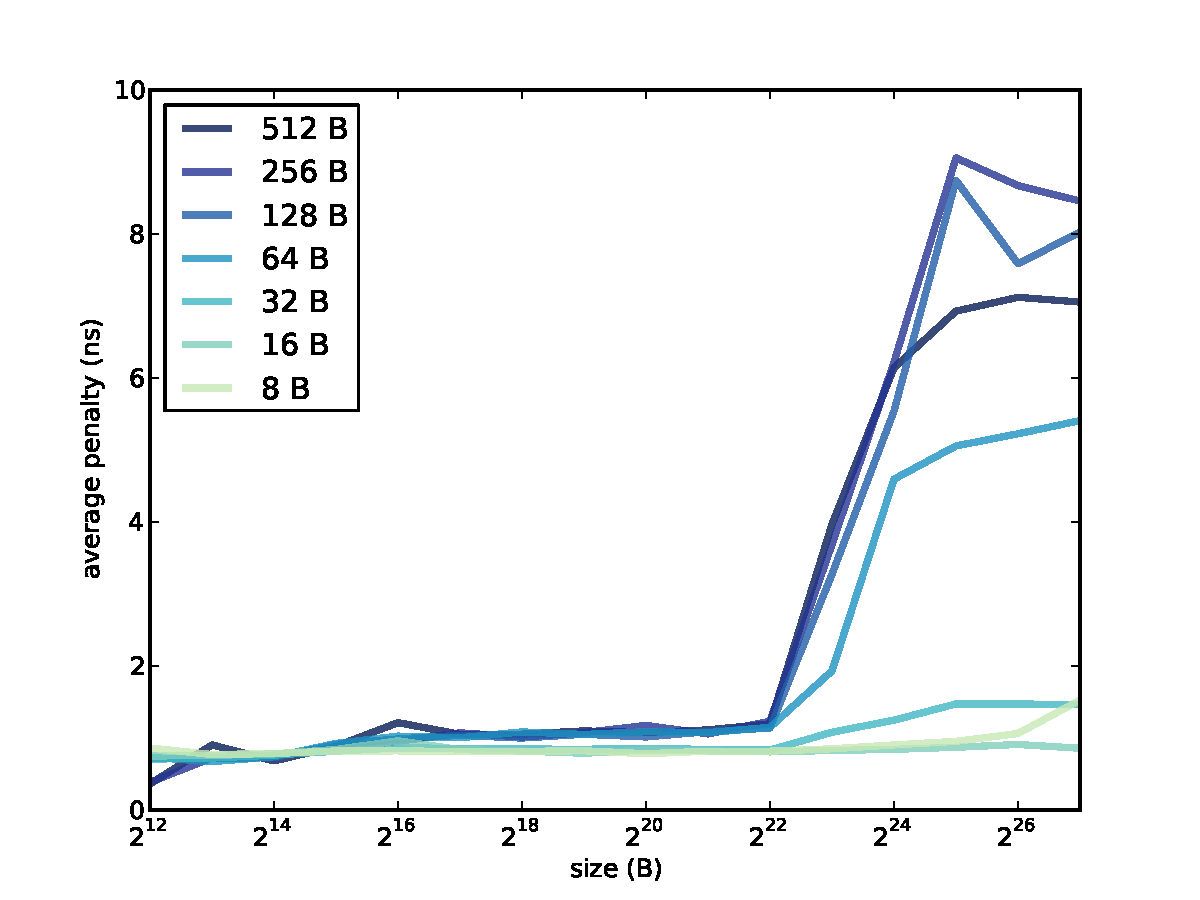
\includegraphics[width=3in]{figs/cache_data.pdf}}
\caption{Average miss penalty as a function of array size and stride.}
\label{cachedata}
\end{figure}

To isolate the time to access the elements of the array,
the program runs a second loop that is almost identical except
that the inner loop doesn't touch the array; it always increments
the same variable:

\begin{verbatim}
    iters2 = 0;
    do {
        sec0 = get_seconds();
        
        for (index = 0; index < limit; index += stride) 
            temp = temp + index;
        
        iters2 = iters2 + 1;
        sec = sec - (get_seconds() - sec0);

    } while (iters2 < iters);
\end{verbatim}

The second loop runs the same number of iterations as the first.
After each iteration, it {\em subtracts} the elapsed time from
{\tt sec}.  When the loop completes, {\tt sec} contains the total
time for all array accesses, minus the total time it took to increment
{\tt temp}.  This difference is the total miss penalty incurred by
all accesses.  Finally, we divide by the number of accesses to
get the average miss penalty per access, in ns:

\begin{verbatim}
sec * 1e9 / iters / limit * stride
\end{verbatim}

If you compile and run {\tt cache.c} you should see output like this:

\begin{verbatim}
Size:    4096 Stride:       8 read+write: 0.8633 ns
Size:    4096 Stride:      16 read+write: 0.7023 ns
Size:    4096 Stride:      32 read+write: 0.7105 ns
Size:    4096 Stride:      64 read+write: 0.7058 ns
\end{verbatim}

If you have Python and {\tt matplotlib} installed, you can use
\verb"graph_data.py" to graph the results.  Figure~\ref{cachedata}
shows the results when I ran it on a Dell Optiplex 7010.
Notice that the array size and stride are reported in
bytes, not number of array elements.

Take a minute to consider this graph, and see what you can infer
about the cache.  Here are some things to think about:

\begin{itemize}

\item The program reads through the array many times, so it has plenty
  of temporal locality.  If the entire array fits in cache, we expect
  the average miss penalty to be near 0.

\item When the stride is 4 bytes, we read every element of the array,
  so the program has plenty of spatial locality.  If the block size is
  big enough to contain 64 elements, for example, the hit rate would
  be 63/64, even if the array does not fit in cache.

\item If the stride is equal to the block size (or greater), the
  spatial locality is effectively zero, because each time we read a
  block, we only access one element.  In that case we expect to see
  the maximum miss penalty.

\end{itemize}

In summary, we expect good cache performance if the array is smaller
than the cache size {\em or} if the stride is smaller than the block
size.  Performance only degrades if the array is bigger than the
cache {\em and} the stride is large.

In Figure~\ref{cachedata}, cache performance is good, for all strides,
as long as the array is less than $2^{22}$ B.  We can infer that the
cache size is near 4 MiB; in fact, according to the specs, it is 3
MiB.

When the stride is 8, 16, or 32 B, cache performance is good.  At 64 B
it starts to degrade, and for larger strides the average miss
penalty is about 9 ns.  We can infer that the block size near 128 B.

Many processors use ``multi-level caches'' that include a small,
fast cache and a bigger, slower cache.  In this example, it looks 
like the miss penalty increases a little when the array size is bigger
than $2^{14}$ B, so it's possible that this processor also has a 16 KB
cache with an access time less than 1 ns.


\section{Programming for cache performance}

Memory caching is implemented in hardware, so most of the time
programmers don't need to know much about it.  But if you know how
caches work, you can write programs that use them more effectively.

For example, if you are working with a large array, it might be
faster to traverse the array once, performing several operations with
each element, rather than traversing the array several times.

If you are working with a 2-D array, it might be stored as an array
of rows.  If you traverse through the elements, it would be faster
to go row-wise, with stride equal to the element size, rather
than column-wise, with stride equal to the row length.

Linked data structures don't always exhibit spatial locality, because
the nodes aren't necessarily contiguous in memory.  But if you allocate
many nodes at the same time, they are usually co-located in the heap.
Or, even better, if you allocate an array of nodes all at once, you
know they will be contiguous.

Recursive strategies like mergesort often have good cache behavior
because they break big arrays into smaller pieces and then work
with the pieces.  Sometimes these algorithms can be tuned to take
advantage of cache behavior.

For applications where performance is critical, it is possible
to design algorithms tailored to the size of the cache, the block size,
and other hardware characterstics.  Algorithms like that are
called ``cache-aware''.  The obvious drawback of cache-aware
algorithms is that they are hardware-specific.


\section{The memory hierarchy}

At some point during this chapter, a question like the following
might have occurred to you: ``If caches are so much faster than
main memory, why not make a really big cache and forget about
memory?''

Without going too far into computer architecture, there are two
reasons: electronics and economics.  Caches are fast because they are
small and close to the CPU, which minimizes delays due to capacitance
and signal propagation.  If you make a cache big, it will be slower.

Also, caches take up space on the processor chip, and bigger chips are
more expensive.  Main memory is usually dynamic random-access memory
(DRAM), which uses only one transistor and one capacitor per bit, so
it is possible to pack more memory into the same amount of space.  But
this way of implementing memory is slower than the way caches are
implemented.
 
Also main memory is usually packaged in a dual in-line memory module
(DIMM) that includes 16 or more chips.  Several small chips are cheaper
than one big one.

The trade-off between speed, size, and cost is the fundamental reason
for caching.  If there were one memory technology that was fast,
big, and cheap, we wouldn't need anything else.

The same principle applies to storage as well as memory.  Solid state drives (SSD) are fast, but they are more expensive than hard drives (HDD), so they tend to be smaller.  Tape drives are even slower than hard
drives, but they can store large amounts of data relatively
cheaply.

The following table shows typical access times, sizes, and 
costs for each of these technologies.  

\vspace{0.1in}
\begin{center}
    \begin{tabular}{| l | l | l | l |}
    \hline
    Device   &   Access   &   Typical    &   Cost   \\
             &   time     &   size       &          \\ \hline
    Register &   0.5 ns   &   256 B      &   ?      \\ \hline
    Cache    &   1 ns     &   2 MiB      &   ?      \\ \hline
    DRAM     &   10 ns    &   4 GiB      &   \$10 / GiB       \\ \hline
    SSD      &   10 \mus  &   100 GiB    &   \$1 / GiB      \\ \hline
    HDD      &   5 ms     &   500 GiB    &   \$0.25 / GiB     \\ \hline
    Tape     &   minutes  &   1--2 TiB   &   \$0.02 / GiB      \\ \hline
    \end{tabular}
\end{center}
\vspace{0.1in}

The number and size of registers depends on details of the
architecture.  Current computers have about 32 general-purpose
registers, each storing one ``word''.  On a 32-bit computer, a word
is 32 bits or 4 B.  On a 64-bit computer, a word is 64 bits or 8 B.
So the total size of the register file is 100--300 B.

The cost of registers and caches is hard to quantify.  They contribute
to the cost of the chips they are on, but consumers don't see that
cost directly.

For the other numbers in the table, I looked at the specifications for
typical hardware for sale from online computer hardware stores.  By
the time you read this, these numbers will be obsolete, but they give
you an idea of what the performance and cost gaps looked like at one
point in time.

These technologies make up the ``memory hierarchy'' (note that this
use of ``memory'' also includes storage).  Each
level of the hierarchy is bigger and slower than the one above it.
And in some sense, each level acts as a cache for the one below
it.  You can think of main memory as a cache for programs and data
that are stored permanently on SSDs and HHDs.  And if you are working
with very large datasets stored on tape, you could use hard drives
to cache one subset of the data at a time.


\section{Caching policy}

The memory hierarchy suggests a framework for thinking about
caching.  At every level of the hierarchy, we have to address
four fundamental questions of caching:

\begin{itemize}

\item Who moves data up and down the hierarchy?  At the top of the
  hierarchy, register allocation is usually done by the compiler.
  Hardware on the CPU handles the memory cache.  Users implicitly move
  data from storage to memory when they execute programs and open
  files.  But the operating system also moves data back and forth
  between memory and storage.  At the bottom of the hierarchy,
  administrators move data explicitly between disk and tape.

\item What gets moved?  In general, block sizes are small at the top
  of the hierarchy and bigger at the bottom.  In a memory cache, a
  typical block size is 128 B.  Pages in memory might be 4 KiB, but
  when the operating system reads a file from disk, it might read 10s
  or 100s of blocks at a time.

\item When does data get moved?  In the most basic cache, data gets
  moved into cache when it is used for the first time.  But many
  caches use some kind of ``prefetching'', meaning that data is
  loaded before it is explicitly requested.  We have already seen
  one form of prefetching: loading an entire block when only part of
  it is requested.

\item Where in the cache does the data go?  When the cache is full, we
  can't bring anything in without kicking something out.  Ideally,
  we want to keep data that will be used again soon and replace data
  that won't.

\end{itemize}

The answers to these questions make up the ``cache policy''.
Near the top of the hierarchy, cache policies tend to be simple
because they have to be fast and they are implemented in hardware.
Near the bottom of the hierarchy, there is more time to make decisions,
and well-designed policies can make a big difference.

Most cache policies are based on the principle that history repeats
itself; if we have information about the recent past, we can use it to
predict the immediate future.  For example, if a block of data has
been used recently, we expect it to be used again soon.  This
principle suggests a replacement policy called ``least recently
used,'' or LRU, which removes from the cache a block of data that
has not been used recently.  For more on this topic, see
\url{http://en.wikipedia.org/wiki/Cache_algorithms}.


\section{Paging}
\label{paging}

In systems with virtual memory, the operating system can move
pages back and forth between memory and storage.  As I mentioned
in Section~\ref{leak}, this mechanism is called ``paging'' or
sometimes ``swapping''.

Here's how the process works:

\begin{enumerate}

\item Suppose Process A calls {\tt malloc} to allocate a chunk.  If there
is no free space in the heap with the requested size, {\tt malloc} calls
{\tt sbrk} to ask the operating system for more memory.

\item If there is a free page in physical memory, the operating system
adds it to the page table for Process A, creating a new range of valid
virtual addresses.

\item If there are no free pages, the paging system chooses a ``victim
page'' belonging to Process B.  It copies the contents of the victim
page from memory to disk, then it modifies the page table for Process
B to indicate that this page is ``swapped out''.

\item Once the data from Process B is written, the page can be reallocated
to Process A.  To prevent Process A from reading Process B's data, the
page should be cleared.

\item At this point the call to {\tt sbrk} can return, giving {\tt malloc}
additional space in the heap.  Then {\tt malloc} allocates the requested
chunk and returns.  Process A can resume.

\item When Process A completes, or is interrupted, the scheduler might
allow Process B to resume.  When Process B accesses a page that has been swapped out, the memory management unit notices that the page is ``invalid'' and causes an interrupt.

\item When the operating system handles the interrupt, it sees that
the page is swapped out, so it transfers the page back from disk to
memory.  

\item Once the page is swapped in, Process B can resume.

\end{enumerate}

When paging works well, it can greatly improve the utilization of
physical memory, allowing more processes to run in less space.
Here's why:

\begin{itemize}

\item Most processes don't use all of their allocated memory.  Many
  parts of the text segment are never executed, or execute once and
  never again.  Those pages can be swapped out without causing any
  problems.

\item If a program leaks memory, it might leave allocated space behind
  and never access it again.  By swapping those pages out, the
  operating system can effectively plug the leak.

\item On most systems, there are processes like daemons that sit idle
  most of the time and only occasionally ``wake up'' to respond to
  events.  While they are idle, these processes can be swapped out.

\item A user might have many windows open, but only a few are active
  at a time.  The inactive processes can be swapped out.

\item Also, there might be many processes running the same program.
  These processes can share the same text and static segments, avoiding the need to keep multiple copies in physical memory.

\end{itemize}

If you add up the total memory allocated to all processes, it can
greatly exceed the size of physical memory, and yet the system can
still behave well.

Up to a point.

When a process accesses a page that's swapped out, it has to get the
data back from disk, which can take several milliseconds.  The
delay is often noticeable.  If you leave a window idle for a long
time and then switch back to it, it might start slowly,
and you might hear the disk drive working while pages are
swapped in.  

Occasional delays like that might be acceptable, but if you have too
many processes using too much space, they start to interfere with each
other.  When Process A runs, it evicts the pages Process B needs.
Then when B runs, it evicts the pages A needs.  When this happens,
both processes slow to a crawl and the system can become unresponsive.
This scenario is called ``thrashing''.

In theory, operating systems could avoid thrashing by detecting an
increase in paging and blocking or killing processes until the system
is responsive again.  But as far as I can tell, most systems don't do
this, or don't do it well; it is often left to users to limit their
use of physical memory or try to recover when thrashing occurs.


\chapter{Multitasking}

In many current systems, the CPU contains multiple cores, which means
it can run several processes at the same time.  In addition, each core
is capable of ``multitasking'', which means it can switch from one
process to another quickly, creating the illusion that many processes
are running at the same time.

The part of the operating system that implements multitasking is
the ``kernel''.  In a nut or seed, the kernel is the innermost
part, surrounded by a shell.  In an operating system, the kernel
is the lowest level of software, surrounded by several other
layers, including an interface called a ``shell.''  Computer
scientists love extended metaphors.

At its most basic, the kernel's job is to
handle interrupts.  An ``interrupt'' is an event that stops the
normal instruction cycle and causes the flow of execution to jump to a
special section of code called an ``interrupt handler''.

%TODO: put new vocab in bold and add glossaries

A {\bf hardware interrupt} is caused when a device sends a signal to the
CPU.  For example, a network interface might cause an interrupt when
a packet of data arrives, or a disk drive might cause an interrupt
when a data transfer is complete.  Most systems also have timers that
cause interrupts at regular intervals, or after an elapsed time.

A {\bf software interrupt} is caused by a running program.  For example, if
an instruction cannot complete for some reason, it might trigger an
interrupt so the condition can be handled by the operating system.
Some floating-point errors, like division by zero, are handled
using interrupts.

When a program needs to access a hardware device,
it makes a {\bf system call}, which is similar to a function call,
except that instead of jumping to the beginning of the function,
it executes a special instruction that triggers an interrupt, causing
the flow of execution to jump to the kernel.  The kernel reads the
parameters of the system call, performs the requested operation,
and then resumes the interrupted process.


\section{Hardware state}

Handling interrupts requires cooperation between hardware and
software.  When an interrupt occurs, there might be several
instructions running on the CPU, data stored in registers, and
other {\bf hardware state}.

Usually the hardware is responsible for bringing the CPU
to a consistent state; for example, every instruction should either
complete or behave as if it never started.  No instruction should
be left half complete.  Also, the hardware is responsible for
saving the program counter (PC), so the kernel knows where to
resume.

Then, usually, it is the responsibility of the interrupt handler
to save the rest of the hardware state before it does anything that
might modify it, and then restore the saved state before the interrupted
process resumes.

Here is an outline of this sequence of events:

\begin{enumerate}

\item When the interrupt occurs, the hardware saves the program
counter in a special register and jumps to the appropriate interrupt
handler.

\item The interrupt handler stores the program counter and the
status register in memory, along with the contents of any data
registers it plans to use.

\item The interrupt handler runs whatever code is needed to handle
the interrupt.

\item Then it restores the contents of the saved registers.  Finally,
it restores the program counter of the interrupted process, which
has the effect of jumping back to the interrupted instruction.

\end{enumerate}

If this mechanism works correctly, there is generally no way for
the interrupted process to know there was an interrupt, unless
it detects the change in time between instructions.


\section{Context switching}

Interrupt handlers can be fast because they don't have to save the
entire hardware state; they only have to save registers they are
planning to use.

But when an interrupt occurs, the kernel does not always resume the
interrupted process.  It has the option of switching to another
process.  This mechanism is called a ``context switch''.

In general, the kernel doesn't know which registers a process will
use, so it has to save all of them.  Also, when it switches to a new
process, it might have to clear data stored in the memory management
unit (see
Section~\ref{address_translation}).  And after the context switch, it
might take some time for the new process to load data into the cache.
For these reasons, context switches are relatively slow, on the order
of thousands of cycles, or a few microseconds.

In a multi-tasking system, each process is allowed to run for a short
period of time called a ``time slice'' or ``quantum''.  During
a context switch, the kernel sets a hardware timer that causes
an interrupt at the end of the time slice.  When the interrupt
occurs, the kernel can switch to another process or allow the
interrupted process to resume.  The part of the operating system
that makes this decision is the ``scheduler''.


\section{The process life cycle}

When a process is created, the operating system allocates a
data structure that contains information about the process, called
a ``process control block'' or PCB.  Among other things, the
PCB keeps track of the process state, which is one of:

\begin{itemize}

\item Running, if the process is currently running on a core.

\item Ready, if the process could be running, but isn't, usually because
there are more runnable processes than cores.

\item Blocked, if the process cannot run because it is waiting for
a future event like network communication or a disk read.

\item Done, if the process has completed, but has exit status
information that has not been read yet.

\end{itemize}

Here are the events that cause a process to transition from one state to another:

\begin{itemize}

\item A process is created when the running program executes a system
  call like {\tt fork}.  At the end of the system call, the new
  process is usually ready.  Then the scheduler might resume the
  original process (the ``parent'') or start the new process (the
  ``child'').

\item When a process is started or resumed by the scheduler, its state
  changes from ready to running.

\item When a process is interrupted and the scheduler chooses not
  to let it resume, its state changes from running to ready.

\item If a process executes a system call that cannot complete
  immediately, like a disk request, it becomes blocked
  and the scheduler usually chooses another process.

\item When an operation like a disk request completes, it causes an
  interrupt.  The interrupt handler figures out which process was
  waiting for the request and switches its state from
  blocked to ready.  Then the scheduler may or may not choose to
  resume the unblocked process.

\item When a process calls {\tt exit}, the interrupt handler stores
  the exit code in the PCB and changes the process's state to done.

\end{itemize}


\section{Scheduling}

As we saw in Section~\ref{unixps} there might be hundreds of
processes on a computer, but usually most of them are blocked.  Most
of the time, there are only a few processes that are ready or running.
When an interrupt occurs, the scheduler decides which process to start
or resume.

On a workstation or laptop, the primary goal of the scheduler is to
minimize response time; that is, the computer should respond quickly
to user actions.  Response time is also important on a server, but in
addition the scheduler might try to maximize throughput, which is the
number of requests that complete per unit of time.

Usually the scheduler doesn't have much information about what
processes are doing, so its decisions are based on a few
heuristics:

\begin{itemize}

\item Processes might be limited by different resources.  A process
that does a lot of computation is probably CPU-bound, which means that
its run time depends on how much CPU time it gets.  A process that
reads data from a network or disk might be I/O-bound, which means that
it would run faster if data input and output went faster, but would not
run faster with more CPU time.  Finally, a process that interacts with
the user is probably blocked, most of the time, waiting for user actions.

The operating system can sometimes classify processes based on their
past behavior, and schedule them accordingly.  For example, when an
interactive process is unblocked, it should probably run immediately,
because a user is probably waiting for a reply.  On the other hand,
a CPU-bound process that has been running for a long time might be
less time-sensitive.

\item If a process is likely to run for a short time and then make
a blocking request, it should probably run immediately, for two reasons:
(1) if the request takes some time to complete, we should start it as soon
as possible, and (2) it is better for a long-running process to wait
for a short one, rather than the other way around.

As an analogy, suppose you are making an apple pie.  The crust takes
5 minutes to prepare, but then it has to chill for half an hour.  It takes
20 minutes to prepare the filling.  If you prepare the crust first,
you can prepare the filling while the crust is chilling, and you can
finish the pie in 35 minutes.  If you prepare the filling first, the
process takes 55 minutes.

\end{itemize}

Most schedulers use some form of priority-based scheduling,
where each process has a priority that can be adjusted up or down
over time.  When the scheduler runs, it chooses the runnable process
with the highest priority.

Here are some of the factors that determine a process's priority:

\begin{itemize}

\item A process usually starts with a relatively high priority so it
  starts running quickly.

\item If a process makes a request and blocks before its time slice is
  complete, it is more likely to be interactive or I/O-bound, so its
  priority should go up.

\item If a process runs for an entire time slice, it is more likely to
  be long-running and CPU-bound, so its priority should go down.

\item If a task blocks for a long time and then becomes ready, it
  should get a priority boost so it can respond to whatever it was
  waiting for.

\item If process A is blocked waiting for process B, for example if
  they are connected by a pipe, the priority of process B should go
  up.

\item The system call {\tt nice} allows a process to decrease (but not
  increase) its own priority, allowing programmers to pass explicit
  information to the scheduler.

\end{itemize}

For most systems running normal workloads, scheduling algorithms
don't have a substantial effect on performance.  Simple scheduling
policies are usually good enough.


\section{Real-time scheduling}

However, for programs that interact with the real world, scheduling
can be very important.  For example, a program that reads data from
sensors and controls motors might have to complete recurring tasks at
some minimum frequency and react to external events with some maximum
response time.  These requirements are often expressed in terms of
``tasks'' that must be completed before ``deadlines''.

Scheduling tasks to meet deadlines is called ``real-time
  scheduling''.  For some applications, a general-purpose operating
system like Linux can be modified to handle real-time scheduling.
These modifications might include:

\begin{itemize}

\item Providing richer APIs for controlling task priorities.

\item Modifying the scheduler to guarantee that the process with
highest priority runs within a fixed amount of time.

\item Reorganizing interrupt handlers to guarantee
a maximum completion time.

\item Modifying locks and other synchronization mechanisms (coming up
  in the next chapter) to allow a high-priority task to preempt a
  lower-priority task.

\item Choosing an implementation of dynamic memory allocation that
guarantees a maximum completion time.

\end{itemize}

For more demanding applications, especially in domains where real-time
response is a matter of life and death, ``real-time operating
  systems'' provide specialized capabilities, often with much simpler
designs than general purpose operating systems.

%TODO: kernel mode?  signals?  user and system time


\chapter{Threads}

When I mentioned threads in Section~\ref{unixps}, I said that a thread
is a kind of process.  Now I will provide a more careful explanation.

When you create a process, the operating system creates a new address
space, which includes the text segment, static segment, and heap; it
also creates a new ``thread of execution'', which includes the program
counter and other hardware state, and the call stack.

The processes we have seen so far are ``single-threaded'', which means
that only one thread of execution runs in each address space.  In this
chapter, you will learn about ``multi-threaded'' processes that have
multiple threads running in the same address space.

Within a single process, all threads share the same text segment, so
they run the same code.  But different threads often run different parts
of the code.

And they share the same static segment, so if one thread changes a
global variable, other threads see the change.  They also share the heap,
so threads can share dynamically-allocated chunks.

But each thread has its own stack, so threads can call functions without
interfering with each other.  Usually threads don't access each
other's local variables (and sometimes they can't).

The example code for this chapter is in the repository for this book,
in a directory named {\tt counter}.  For information on downloading
this code, see Section~\ref{code}.


\section{Creating threads}

The most popular threading standard used with C is POSIX Threads, or Pthreads for short.  The POSIX standard defines a thread model and an interface for creating and controlling threads.  Most versions of UNIX provide an implementation of Pthreads.

Using Pthreads is like using most C libraries:

\begin{itemize}

\item You include headers files at the beginning of your
program.

\item You write code that calls functions defined by Pthreads.

\item When you compile the program, you link it with the Pthread library.

\end{itemize}

For my examples, I include the following headers:

\begin{verbatim}
#include <stdio.h>
#include <stdlib.h>
#include <pthread.h>
#include <semaphore.h>
\end{verbatim}

The first two are standard; the third is for Pthreads and
the fourth is for semaphores.  To compile with the Pthread library in {\tt gcc}, you can use the {\tt -l} option on the command line:

\begin{verbatim}
gcc -g -O2 -o array array.c -lpthread
\end{verbatim}

This compiles a source file named {\tt array.c} with debugging info
and optimization, links with the Pthread library, and generates an
executable named {\tt array}.


\section{Creating threads}

The Pthread function that creates threads is called \verb"pthread_create".
The following function shows how to use it:

\begin{verbatim}
pthread_t make_thread(void *(*entry)(void *), Shared *shared)
{
    int n;
    pthread_t thread;

    n = pthread_create(&thread, NULL, entry, (void *)shared);
    if (n != 0) {
        perror("pthread_create failed");
        exit(-1);
    }
    return thread;
}
\end{verbatim}

\verb"make_thread" is a wrapper I wrote to make
\verb"pthread_create" easier to use, and to provide error-checking.

%TODO: Define a newcommand like \py to make verb easier to use, and
% get rid of the \_ hockey sticks

The return type from \verb"pthread_create" is \verb"pthread_t",
which you can think of as an id or ``handle'' for the new thread.  

If {\tt pthread\_create} succeeds, it returns 0 and \verb"make_thread"
returns the handle of the new thread.
If an error occurs, {\tt pthread\_create} 
returns an error code and \verb"make_thread" prints an error message
and exits.

The parameters of {\tt pthread\_create} take some
explaining.  Starting with the second, {\tt Shared}
is a structure I defined to contain values shared between threads.
The following {\tt typedef} statement creates the new type:

\begin{verbatim}
typedef struct {
    int counter;
} Shared;
\end{verbatim}

In this case, the only shared variable is {\tt counter}.
{\tt make\_shared} allocates
space for a {\tt Shared} structure and initializes the contents:

\begin{verbatim}
Shared *make_shared()
{
    Shared *shared = check_malloc(sizeof (Shared));
    shared->counter = 0;
    return shared;
}
\end{verbatim}

Now that we have a shared data structure, let's get back to
{\tt pthread\_create}.
The third parameter is a pointer to a function that takes
a {\tt void} pointer and returns a {\tt void} pointer.  If the syntax
for declaring this type makes your eyes bleed, you are not alone.
Anyway, the purpose of this parameter is to specify the function where
the execution of the new thread will begin.  By convention, this
function is named {\tt entry}:

\begin{verbatim}
void *entry(void *arg)
{
    Shared *shared = (Shared *) arg;
    child_code(shared);
    pthread_exit(NULL);
}
\end{verbatim}

The parameter of {\tt entry} has to be declared as a {\tt void}
pointer, but in this program we know that it is really a pointer to a
{\tt Shared} structure, so we can typecast it accordingly and then
pass it along to {\tt child\_code}, which does the real work.

As a simple example, \verb"child_code" prints the value of
the shared counter and increments it.

\begin{verbatim}
void child_code(Shared *shared)
{  
    printf("counter = %d\n", shared->counter);
    shared->counter++;
}
\end{verbatim}

When {\tt child\_code} returns, {\tt entry} invokes
\verb"pthread_exit" which can be used to pass a value to the thread
that joins with this thread.  In this case, the child has nothing to
say, so we pass {\tt NULL}.

Finally, here is the code that creates the child threads:

\begin{verbatim}
    int i;
    pthread_t child[NUM_CHILDREN];

    Shared *shared = make_shared(1000000);

    for (i=0; i<NUM_CHILDREN; i++) {
        child[i] = make_thread(entry, shared);
    }
\end{verbatim}

\verb"NUM_CHILDREN" is a compile-time constant that determines
the number of child threads.  {\tt child} is an array of
thread handles.


\section{Joining threads}

When one thread wants to wait for another thread to complete,
it invokes {\tt pthread\_join}.
Here is my wrapper for {\tt pthread\_join}:

\begin{verbatim}
void join_thread(pthread_t thread)
{
    int ret = pthread_join(thread, NULL);
    if (ret == -1) {
      perror("pthread_join failed");
      exit(-1);
    }
}
\end{verbatim}

The parameter is the handle of the thread you want to wait for.
All the wrapper does is call {\tt pthread\_join} and check the
result.

Any thread can join any other thread, but in the most common pattern
the parent thread creates and joins all child threads.
Continuing the example from the previous section, here's the
code that waits on the children:

\begin{verbatim}
    for (i=0; i<NUM_CHILDREN; i++) {
        join_thread(child[i]);
    }
\end{verbatim}

This loops waits for the children one at a time in the order they
were created.  There is no guarantee that the child threads complete 
in that order, but this loop works correctly even if they don't.  If one
of the children is late, the loop might have to wait, and other children
might complete in the meantime.  But regardless, the loop exits
only when all children are done.

If you have downloaded the repository for this book (see
Section~\ref{code}), you'll find this example in {\tt
  counter/counter.c}.  You can compile and run it like this:

\begin{verbatim}
$ make counter
gcc -Wall counter.c -o counter -lpthread
$ ./counter
\end{verbatim}

When I ran it with 5 children, I got the following output:

\begin{verbatim}
counter = 0
counter = 0
counter = 1
counter = 0
counter = 3
\end{verbatim}

When you run it, you will probably get different results.  And if
you run it again, you might get different results each time.  What's
going on?


\section{Synchronization errors}

The problem with the previous program is that the children
access the shared variable, {\tt counter}, without synchronization,
so several threads can read the same value of {\tt counter} before
any threads increment it.

Here is a sequence of events that could explain the output in the
previous section:

\begin{verbatim}
Child A reads 0
Child B reads 0
Child C reads 0
Child A prints   0
Child B prints   0
Child A sets counter=1
Child D reads 1
Child D prints   1
Child C prints   0
Child A sets counter=1
Child B sets counter=2
Child C sets counter=3
Child E reads 3
Child E prints   3
Child D sets counter=4
Child E sets counter=5
\end{verbatim}

Each time you run the program, threads might be interrupted at different
points, or the scheduler might choose different threads to run, so
the sequence of events, and the results, will be different.

Suppose we want to impose some order.  For example, we might want
each thread to read a different value of {\tt counter} and increment
it, so that the value of {\tt counter} reflects the number of
threads that have executed \verb"child_code".

To enforce that requirement, we can use a ``mutex'', which is
an object that guarantees ``mutual exclusion'' for a block of code;
that is, only one thread can execute the block at a time.

I have written a small module called {\tt mutex.c} that provides
mutex objects.  I'll show you how to use it first; then I'll explain
how it works.

Here's a version of \verb"child_code" that uses a mutex to synchronize
threads:

\begin{verbatim}
void child_code(Shared *shared)
{
    mutex_lock(shared->mutex);
    printf("counter = %d\n", shared->counter);
    shared->counter++;
    mutex_unlock(shared->mutex);
}
\end{verbatim}

Before any thread can access {\tt counter}, it has to ``lock''
the mutex, which has the effect of barring all other threads.
Suppose Thread A has locked the mutex and is in the
middle of \verb"child_code".  If Thread B arrives and
executes \verb"mutex_lock", it blocks.

When Thread A is done, it executes \verb"mutex_unlock",
which allows Thread B to proceed.  In effect, the threads
line up to execute \verb"child_code" one at a time, so they
can't interfere with each other.  When I run this code with
5 children, I get:

\begin{verbatim}
counter = 0
counter = 1
counter = 2
counter = 3
counter = 4
\end{verbatim}

And that satisfies the requirements.  In order for this solution to
work, I have to add the Mutex to the Shared struct:

\begin{verbatim}
typedef struct {
    int counter;
    Mutex *mutex;
} Shared;
\end{verbatim}

And initialize it in \verb"make_shared"

\begin{verbatim}
Shared *make_shared(int end)
{
    Shared *shared = check_malloc(sizeof(Shared));
    shared->counter = 0;
    shared->mutex = make_mutex();   //-- this line is new
    return shared;
}
\end{verbatim}

The code in this section is in \verb"counter_mutex.c".
The definition of {\tt Mutex} is in {\tt mutex.c}, which I
explain in the next section.



\section{Mutex}

My definition of {\tt Mutex} is a wrapper for a type called
\verb"pthread_mutex_t", which is defined in the POSIX threads API.

To create a POSIX mutex, you have to allocate space for a
\verb"pthread_mutex_t" type and then call \verb"pthread_mutex_init".

One of the problems with this API is that \verb"pthread_mutex_t"
behaves like a structure, so if you pass it as an argument, it makes a
copy, which makes the mutex behave incorrectly.  To avoid that, you have to
pass \verb"pthread_mutex_t" by address.

My code makes it easier to get that right.  It defines a
type, {\tt Mutex}, which is just a more readable name for
\verb"pthread_mutex_t":

\begin{verbatim}
#include <pthread.h>

typedef pthread_mutex_t Mutex;
\end{verbatim}

Then it defines \verb"make_mutex", which allocates space and
initializes the mutex:

\begin{verbatim}
Mutex *make_mutex()
{
    Mutex *mutex = check_malloc(sizeof(Mutex));
    int n = pthread_mutex_init(mutex, NULL);
    if (n != 0) perror_exit("make_lock failed"); 
    return mutex;
}
\end{verbatim}

The return value is a pointer, which you can pass around as an
argument without causing unwanted copying.

The functions to lock and unlock the mutex are simple wrappers
for POSIX functions:

\begin{verbatim}
void mutex_lock(Mutex *mutex)
{
    int n = pthread_mutex_lock(mutex);
    if (n != 0) perror_exit("lock failed");
}

void mutex_unlock(Mutex *mutex)
{
    int n = pthread_mutex_unlock(mutex);
    if (n != 0) perror_exit("unlock failed");
}
\end{verbatim}

This code is in {\tt mutex.c} and the header file {\tt mutex.h}.


\chapter{Condition variables}
\label{csem}

Many simple synchronization problems can be solved using mutexes
as shown in the previous chapter.  In this chapter I introduce a
bigger challenge, the well-known ``Producer-Consumer problem'', and
a new tool to solve it, the condition variable.

\section{The work queue}
\label{queue}

In some multi-threaded programs, threads are organized to perform
different tasks.  Often they communicate with each other using a queue,
where some threads, called ``producers'', put data into the queue
and other threads, called ``consumers'', take data out.

For example, in applications with a graphical user interface, there
might be one thread that runs the GUI, responding to user events,
and another thread that processes user requests.  In that case,
the GUI thread might put requests into a queue and the ``back end''
thread might take requests out and process them.

To support this organization, we need a queue implementation that
is ``thread safe'', which means that both threads (or more than two)
can access the queue at the same time.  And we need to handle at least
one special case, when the queue is empty; and, if the size of the
queue is bounded, when the queue is full.

I'll start with a simple queue that is not thread safe, then we'll see
what goes wrong and fix it.  The code for this example is in the
repository for this book, in a folder called {\tt queue}.  The file
{\tt queue.c} contains a basic implementation of a circular buffer,
which you can read about at
\url{https://en.wikipedia.org/wiki/Circular_buffer}.

Here's the structure definition:

\begin{verbatim}
typedef struct {
    int *array;
    int length;
    int next_in;
    int next_out;
} Queue;
\end{verbatim}

{\tt array} is the array that contains the elements of the queue.
For this example the elements are ints, but more generally
they would be structures that contain user events, items of work, etc.

{\tt length} is the length of the array.  \verb"next_in" is an
index into the array that indices where the next element should be
added; similarly, \verb"next_out" is the index of the next element
that should be removed.

\verb"make_queue" allocates space for this structure and initializes
the fields:

\begin{verbatim}
Queue *make_queue(int length)
{
    Queue *queue = (Queue *) malloc(sizeof(Queue));
    queue->length = length;
    queue->array = (int *) malloc(length * sizeof(int));
    queue->next_in = 0;
    queue->next_out = 0;
    return queue;
}
\end{verbatim}

The initial value for \verb"next_out" needs some explaining.
Since the queue is initially empty, there is no next element to
remove, so \verb"next_out" is invalid.  Setting
\verb"next_out == next_in" is a special case that indicates
that the queue is empty, so we can write:

\begin{verbatim}
int queue_empty(Queue *queue)
{
    return (queue->next_in == queue->next_out);
}
\end{verbatim}

Now we can add elements to the queue using \verb"queue_push":

\begin{verbatim}
void queue_push(Queue *queue, int item) {
    if (queue_full(queue)) {
        perror_exit("queue is full");
    }
  
    queue->array[queue->next_in] = item;
    queue->next_in = queue_incr(queue, queue->next_in);
}
\end{verbatim}

If the queue is full, \verb"queue_push" prints an error message
and exits.  I will explain \verb"queue_full" soon.

If the queue is not full, \verb"queue_push" inserts the new
element and then increments \verb"next_in" using \verb"queue_incr":

\begin{verbatim}
int queue_incr(Queue *queue, int i)
{
    return (i+1) % queue->length;
}
\end{verbatim}

When the index, {\tt i}, gets to the end of the array, it wraps around
to 0.  And that's where we run into a tricky part.  If we keep adding
elements to the queue, eventually \verb"next_in" wraps around and catches
up with \verb"next_out".  But if \verb"next_in == next_out", we would
incorrectly conclude that the queue was empty.

To avoid that, we define another special case to indicate that the
queue is full:

\begin{verbatim}
int queue_full(Queue *queue)
{
    return (queue_incr(queue, queue->next_in) == queue->next_out);
}
\end{verbatim}

If incrementing \verb"next_in" lands on \verb"next_out", that means
we can't add another element without making the queue seem empty.  So
we stop one element before the ``end'' (keeping in mind that the end of
the queue can be anywhere, not necessarily the end of the array).

Now we can write \verb"queue_pop", which removes and returns the next
element from the queue:

\begin{verbatim}
int queue_pop(Queue *queue) {
    if (queue_empty(queue)) {
        perror_exit("queue is empty");
    }
  
    int item = queue->array[queue->next_out];
    queue->next_out = queue_incr(queue, queue->next_out);
    return item;
}
\end{verbatim}

If you try to pop from an empty queue, \verb"queue_pop" prints
an error message and exits.


\section{Producers and consumers}
\label{prodcon}

Now let's make some threads to access this queue.  Here's the
producer code:

\begin{verbatim}
void *producer_entry(void *arg)
{
    int i;
    Shared *shared = (Shared *) arg;

    for (i=0; i<QUEUE_LENGTH-1; i++) {
        printf("adding item %d\n", i);
        queue_push(shared->queue, i);
    }
    pthread_exit(NULL);
}
\end{verbatim}

Here's the consumer code:

\begin{verbatim}
void *consumer_entry(void *arg)
{
    int i;
    int item;
    Shared *shared = (Shared *) arg;

    for (i=0; i<QUEUE_LENGTH-1; i++) {
        item = queue_pop(shared->queue);
        printf("consuming item %d\n", item);
    }
    pthread_exit(NULL);
}
\end{verbatim}

%TODO: switch to c99 and inline the declarations of i

Here's the parent code that starts the threads and waits for them

\begin{verbatim}
    int i;
    pthread_t child[NUM_CHILDREN];

    Shared *shared = make_shared();

    child[0] = make_thread(producer_entry, shared);
    child[1] = make_thread(consumer_entry, shared);

    for (i=0; i<NUM_CHILDREN; i++) {
        join_thread(child[i]);
    }
\end{verbatim}

And finally here's the shared structure that contains the queue:

\begin{verbatim}
typedef struct {
    Queue *queue;
} Shared;

Shared *make_shared()
{
    Shared *shared = check_malloc(sizeof(Shared));
    shared->queue = make_queue(QUEUE_LENGTH);
    return shared;
}
\end{verbatim}

The code we have so far is a good starting place, but it has
several problems:

\begin{itemize}

\item Access to the queue is not thread safe.  Different threads
could access {\tt array}, \verb"next_in", and \verb"next_out"
at the same time and leave the queue in a broken, ``inconsistent''
state.

\item If the consumer is scheduled first, it finds the queue empty,
print an error message, and exits.  We would rather have the consumer
block until the queue is not empty.  Similarly, we would like the
producer to block if the queue is full.

\end{itemize}

In the next section, we solve the first problem with a Mutex.
In the following section, we solve the second problem with condition
variables.


\section{Mutual exclusion}

We can make the queue thread safe with a mutex.  This version
of the code is in \verb"queue_mutex.c".

First we add a Mutex pointer to the queue structure:

\begin{verbatim}
typedef struct {
  int *array;
  int length;
  int next_in;
  int next_out;
  Mutex *mutex;          //-- this line is new
} Queue;
\end{verbatim}

And initialize the Mutex in \verb"make_queue":

\begin{verbatim}
Queue *make_queue(int length)
{
  Queue *queue = (Queue *) malloc(sizeof(Queue));
  queue->length = length;
  queue->array = (int *) malloc(length * sizeof(int));
  queue->next_in = 0;
  queue->next_out = 0;
  queue->mutex = make_mutex();   //-- new
  return queue;
}
\end{verbatim}

Next we add synchronization code to \verb"queue_push":

\begin{verbatim}
void queue_push(Queue *queue, int item) {
  mutex_lock(queue->mutex);   //-- new
  if (queue_full(queue)) {
    mutex_unlock(queue->mutex);   //-- new
    perror_exit("queue is full");
  }
  
  queue->array[queue->next_in] = item;
  queue->next_in = queue_incr(queue, queue->next_in);
  mutex_unlock(queue->mutex);   //-- new
}
\end{verbatim}

Before checking whether the queue is full, we have to lock
the mutex.  If the queue is full, we have to unlock
the mutex before exiting; otherwise the thread would leave
the mutex locked and no other threads could proceed.

The synchronization code for \verb"queue_pop" is similar:

\begin{verbatim}
int queue_pop(Queue *queue) {
  mutex_lock(queue->mutex);
  if (queue_empty(queue)) {
    mutex_unlock(queue->mutex);
    perror_exit("queue is empty");
  }
  
  int item = queue->array[queue->next_out];
  queue->next_out = queue_incr(queue, queue->next_out);
  mutex_unlock(queue->mutex);
  return item;
}
\end{verbatim}

Note that the other Queue functions, \verb"queue_full",
\verb"queue_empty", and \verb"queue_incr" do not try to lock
the mutex.  Any thread that calls these functions is required to
lock the mutex first; this requirement is part of the documented
interface for these functions.

With this additional code, the queue is thread safe; if you run it, you
should not see any synchronization errors.  But it is likely
that the consumer will exit at some point because the queue is
empty, or the producer will exit because the queue is full,
or both.

The next step is to add condition variables.


\section{Condition variables}

A condition variable is a data structure associated with a condition;
it allows threads to block until the condition becomes true.  For
example, \verb"thread_push" might want to check whether the queue is
full and, if so, block until it is not full.  So the ``condition'' we
are interested in is ``queue not full''.

Similarly, \verb"thread_pop" might want to wait for a condition
like ``queue not empty''.

Here's how we can add these capabilities to the queue code.  First
we add two condition variables to the Queue structure:

\begin{verbatim}
typedef struct {
  int *array;
  int length;
  int next_in;
  int next_out;
  Mutex *mutex;
  Cond *nonempty;   //-- new
  Cond *nonfull;    //-- new
} Queue;
\end{verbatim}

And initialize them in \verb"make_queue":

\begin{verbatim}
Queue *make_queue(int length)
{
  Queue *queue = (Queue *) malloc(sizeof(Queue));
  queue->length = length;
  queue->array = (int *) malloc(length * sizeof(int));
  queue->next_in = 0;
  queue->next_out = 0;
  queue->mutex = make_mutex();
  queue->nonempty = make_cond();   //-- new
  queue->nonfull = make_cond();    //-- new
  return queue;
}
\end{verbatim}

Now in \verb"queue_pop", if we find the queue empty, we don't
exit; instead we use the condition variable to block:

\begin{verbatim}
int queue_pop(Queue *queue) {
  mutex_lock(queue->mutex);
  while (queue_empty(queue)) {
    cond_wait(queue->nonempty, queue->mutex);  //-- new
  }
  
  int item = queue->array[queue->next_out];
  queue->next_out = queue_incr(queue, queue->next_out);
  mutex_unlock(queue->mutex);
  cond_signal(queue->nonfull);   //-- new
  return item;
}
\end{verbatim}

\verb"cond_wait" is complicated, so let's take it slow.  
The first argument is the condition variable; in this case,
the condition we are waiting for is ``queue not empty''.  The second
argument is the mutex that protects the queue.  Before you
call \verb"cond_wait", you have to lock the mutex.  Otherwise the
whole thing doesn't work.

When the thread that locked the mutex calls \verb"cond_wait", it
unlocks the mutex and then blocks.  This is important.  If
\verb"cond_wait" did not unlock the mutex before blocking, no
other thread would be able to access the queue, no more items
could be added, and the queue would always be empty.

So while the consumer is blocked on {\tt nonempty}, the producer can
run.  Let's see what happens when the producer runs \verb"queue_push":

\begin{verbatim}
void queue_push(Queue *queue, int item) {
  mutex_lock(queue->mutex);
  while (queue_full(queue)) {
    cond_wait(queue->nonfull, queue->mutex);    //-- new
  }
  
  queue->array[queue->next_in] = item;
  queue->next_in = queue_incr(queue, queue->next_in);
  mutex_unlock(queue->mutex);
  cond_signal(queue->nonempty);  //-- new
}
\end{verbatim}

Let's assume that the queue is not full, so the producer doesn't
run \verb"cond_wait" and doesn't block.  It adds a new element
to the queue and then unlocks the mutex.  But before exiting,
it does one more thing: it ``signals'' the condition variable
{\tt nonempty}.

Signalling a condition variable indicates that the condition is
true, or at least that it might be.  If there are no threads waiting
on the condition variable, the signal has no effect.

If there are threads waiting on the condition variable, one of them
gets unblocked and resumes execution of \verb"cond_wait".  But before
the awakened thread can return from \verb"cond_wait", it has
to wait for and lock the mutex, again.

Now go back to \verb"queue_pop" and see what happens when the thread
returns from \verb"cond_wait".  It loops back to the top of the while
loop and checks the condition again.  I'll explain why in just a
second, but for now let's assume that the condition is true; that is,
the queue is not empty.

When the thread exits the while loop, we know two things: (1) the condition
is true, so there is at least one item in the queue, and (2) the mutex
is locked, so it is safe to access the queue.

After removing an item, \verb"queue_pop" unlocks the mutex, signals
that the queue is not full, and returns.

In the next section I'll show you how my Cond code works, but first I
want to answer two frequently-asked questions:

\begin{itemize}

\item Why is \verb"cond_wait" inside a for loop rather than an if
statement; that is, why do we have to check the condition again after
returning from \verb"cond_wait"?

The primary reason you have to re-check the condition is the possibility
of an intercepted signal.  Suppose Thread A is waiting on {\tt nonempty}.
Thread B adds an item to the queue and signals {\tt nonempty}.  Thread
A wakes up an tries to lock the mutex, but before it gets the chance,
Evil Thread C swoops in, locks the mutex, pops the item from the
queue, and unlocks the mutex.  Now the queue is empty again, but
Thread A is not blocked any more.  Thread A could lock the mutex and
returns from \verb"cond_wait".  If Thread A does not check the condition
again, it would try to pop an element from an empty queue, and probably
cause an error.

\item The other question that comes up when people learn about condition
variables is ``How does the condition variable know what condition it
is associated with?''

This question is understandable because there is no explicit connection
between a Cond structure and the condition it relates to.  The
connection is implicit in the way it is used.

Here's one way to think of it: the condition associated with a Cond
is the thing that is false when you call \verb"cond_wait" and true
when you call \verb"cond_signal".  Of course, there might be many
conditions that are true in the first case and false in the second.
The right one is only in the mind of the programmer, so it should be
explained carefully in the documentation.

\end{itemize}


\section{Condition variable implementation}

The Cond structure I used in the previous section is a wrapper
for a type called \verb"pthread_cond_t", which is defined in the POSIX
threads API.  It is very similar to Mutex, which is a wrapper for
\verb"pthread_mutex_t".  Both wrappers are defined in {\tt utils.c} and
{\tt utils.h}.

Here's the typedef:

\begin{verbatim}
typedef pthread_cond_t Cond;
\end{verbatim}

\verb"make_cond" allocates space, initializes the condition variable,
and returns a pointer:

\begin{verbatim}
Cond *make_cond()
{
  Cond *cond = check_malloc(sizeof(Cond)); 
  int n = pthread_cond_init(cond, NULL);
  if (n != 0) perror_exit("make_cond failed");
 
  return cond;
}
\end{verbatim}

And here are the wrappers for \verb"cond_wait" and \verb"cond_signal".

\begin{verbatim}
void cond_wait(Cond *cond, Mutex *mutex)
{
  int n = pthread_cond_wait(cond, mutex);
  if (n != 0) perror_exit("cond_wait failed");
}

void cond_signal(Cond *cond)
{
  int n = pthread_cond_signal(cond);
  if (n != 0) perror_exit("cond_signal failed");
}
\end{verbatim}

At this point there should be nothing too surprising there.



\chapter{Semaphores in C}

Semaphores are a good way to learn about synchronization, but
they are not as widely used, in practice, as mutexes and
condition variables.

Nevertheless, there are some synchronization problems that can be
solved simply with semaphores, yielding solutions that are more
demonstrably correct.

This chapter presents a C API for working with semaphores and
my code for making it easier to work with.  And it presents
a final challenge: can you write an implementation of a semaphore
using mutexes and condition variables?

The code for this chapter is in directory {\tt semaphore} in the
repository for this book (see Section~\ref{code}).


\section{POSIX Semaphores}

A semaphore is a data structure used to help threads work together
without interfering with each other.

The POSIX standard specifies an interface for semaphores;
it is not part of Pthreads, but most UNIXes
that implement Pthreads also provide semaphores.

POSIX semaphores have type {\tt sem\_t}.  
This type behaves like a structure, so
if you assign it to a variable you are making a copy of the
contents.  Copying a semaphore is almost certainly
a bad idea; in POSIX, the behavior of the copy is undefined.

Fortunately, it is easy to put a wrapper around {\tt sem\_t}
to make it safer and easier to use.  My wrapper API is in {\tt sem.h}:

\begin{verbatim}
typedef sem_t Semaphore;

Semaphore *make_semaphore(int value);
void semaphore_wait(Semaphore *sem);
void semaphore_signal(Semaphore *sem);
\end{verbatim}

{\tt Semaphore} is a synonym for \verb"sem_t", but I find it more
readable, and the capital letter reminds me to treat it like an
object and pass it by pointer.

The implementation of these functions is in {\tt sem.c}:

\begin{verbatim}
Semaphore *make_semaphore(int value)
{
  Semaphore *sem = check_malloc(sizeof(Semaphore));
  int n = sem_init(sem, 0, value);
  if (n != 0) perror_exit("sem_init failed");
  return sem;
}
\end{verbatim}

{\tt make\_semaphore} takes the initial value of the semaphore
as a parameter.  It allocates space for a Semaphore, initializes
it, and returns a pointer to {\tt Semaphore}.

{\tt sem\_init} returns 0 if it succeeds and -1 if anything goes
wrong.  One nice thing about using wrapper functions is that you can
encapsulate the error-checking code, which makes the code that uses
these functions more readable.

Here is the implementation of \verb"semaphore_wait":

\begin{verbatim}
void semaphore_wait(Semaphore *sem)
{
  int n = sem_wait(sem);
  if (n != 0) perror_exit("sem_wait failed");
}
\end{verbatim}

And here is \verb"semaphore_signal":

\begin{verbatim}
void semaphore_signal(Semaphore *sem)
{
  int n = sem_post(sem);
  if (n != 0) perror_exit("sem_post failed");
}
\end{verbatim}

I prefer to call this operation ``signal'' rather than ``post'',
although both terms are common.

Here's an example that shows how to use a semaphore as a mutex:

\begin{verbatim}
Semaphore *mutex = make_semaphore(1);
semaphore_wait(mutex);
// protected code goes here
semaphore_signal(mutex);
\end{verbatim}

When you use a semaphore as a mutex, you usually
initialize it to 1 to indicate
that the mutex is unlocked; that is, one thread can
pass the semaphore without blocking.

Here I am using the variable name {\tt mutex} to indicate that
the semaphore is being used as a mutex.  But remember that the behavior
of a semaphore is not the same as a Pthread mutex.


\section{Producers and consumers with semaphores}

Using these semaphore wrapper functions, we can
write a solution to the Producer-Consumer problem from
Section~\ref{prodcon}.
The code in this section is in \verb"queue_sem.c".

Here's the new definition of {\tt Queue}, replacing the mutex
and condition variables with semaphores:

\begin{verbatim}
typedef struct {
  int *array;
  int length;
  int next_in;
  int next_out;
  Semaphore *mutex;       //-- new
  Semaphore *items;       //-- new
  Semaphore *spaces;      //-- new
} Queue;
\end{verbatim}

And here's the new version of \verb"make_queue":

\begin{verbatim}
Queue *make_queue(int length)
{
  Queue *queue = (Queue *) malloc(sizeof(Queue));
  queue->length = length;
  queue->array = (int *) malloc(length * sizeof(int));
  queue->next_in = 0;
  queue->next_out = 0;
  queue->mutex = make_semaphore(1);
  queue->items = make_semaphore(0);
  queue->spaces = make_semaphore(length-1);
  return queue;
}
\end{verbatim}

{\tt mutex} is used to guarantee exclusive access to the queue;
the initial value is 1, so the mutex is
initially unlocked.

{\tt items} is the number of items in the queue, which is also the number
of consumer threads that can execute \verb"queue_pop" without blocking.
Initially there are no items in the queue.

{\tt spaces} is the number of empty spaces in the queue, which is the
number of producer threads that can execute \verb"queue_push" without
blocking.  Initially the number of spaces is the capacity of the queue,
which is {\tt length-1}, as explained in Section~\ref{queue}.

Here is the new version of \verb"queue_push", which is run by
producer threads:

\begin{verbatim}
void queue_push(Queue *queue, int item) {
  semaphore_wait(queue->spaces);
  semaphore_wait(queue->mutex);

  queue->array[queue->next_in] = item;
  queue->next_in = queue_incr(queue, queue->next_in);

  semaphore_signal(queue->mutex);
  semaphore_signal(queue->items);
}
\end{verbatim}

Notice that \verb"queue_push" doesn't have to call
\verb"queue_full" any more; instead, the semaphore keeps track of
how many spaces are available and blocks producers if the queue
is full.

Here is the new version of \verb"queue_pop":

\begin{verbatim}
int queue_pop(Queue *queue) {
  semaphore_wait(queue->items);
  semaphore_wait(queue->mutex);
  
  int item = queue->array[queue->next_out];
  queue->next_out = queue_incr(queue, queue->next_out);

  semaphore_signal(queue->mutex);
  semaphore_signal(queue->spaces);

  return item;
}
\end{verbatim}

This solution is explained, using pseudo-code, in Chapter 4 of
{\it The Little Book of Semaphores}.

Using the code in the repo for this book, you should be able to compile
and run this solution.  You should be able to run:

\begin{verbatim}
$ make queue_sem
$ ./queue_sem
\end{verbatim}



\section{Make your own semaphores}
\label{makeyourown}

Any problem that can be solved with semaphores can also be solved
with condition variables and mutexes.  One way to prove that's true
is to implement a semaphore using condition variables and mutexes.

Before you go on, you might want to try this as an exercise: write
functions that implement the semaphore API in {\tt sem.h}
using using condition variables and mutexes.  You can put your
solution in {\tt mysem.c} and {\tt mysem.h} in the repo for this book,
and you'll find my solution in \verb"mysem_soln.c" and
\verb"mysem_soln.h".

If you have trouble getting started, you can use the following
structure definition, from my solution, as a hint:

\begin{verbatim}
typedef struct {
  int value, wakeups;
  Mutex *mutex;
  Cond *cond;
} Semaphore;
\end{verbatim}

{\tt value} is the value of the semaphore.  {\tt wakeups} counts
the number of pending signals; that is, the number of threads
that have been woken but have not yet resumed execution.  The reason
for wakeups is to make sure that our semaphores have
Property 3, described in {\tt The Little Book of Semaphores}.

{\tt mutex} provides exclusive access to {\tt value} and
{\tt wakeups}; {\tt cond} is the condition variable threads
wait on if they wait on the semaphore.

Here is the initialization code for this structure:

\begin{verbatim}
Semaphore *make_semaphore(int value)
{
  Semaphore *semaphore = check_malloc(sizeof(Semaphore));
  semaphore->value = value;
  semaphore->wakeups = 0;
  semaphore->mutex = make_mutex();
  semaphore->cond = make_cond();
  return semaphore;
}
\end{verbatim}


\subsection{Semaphore implementation}

Here is my implementation of semaphores using POSIX mutexes
and condition variables:

\begin{verbatim}
void semaphore_wait(Semaphore *semaphore)
{
  mutex_lock(semaphore->mutex);
  semaphore->value--;

  if (semaphore->value < 0) {
    do {
      cond_wait(semaphore->cond, semaphore->mutex);
    } while (semaphore->wakeups < 1);
    semaphore->wakeups--;
  }
  mutex_unlock(semaphore->mutex);
}
\end{verbatim}

When a thread waits on the semaphore, it has to lock the mutex
before it decrements {\tt value}.  If the value of the semaphore
becomes negative, the thread blocks until a ``wakeup'' is
available.  While it is blocked, the mutex is unlocked, so another
thread can signal.

Here is the code for \verb"semaphore_signal":

\begin{verbatim}
void semaphore_signal(Semaphore *semaphore)
{
  mutex_lock(semaphore->mutex);
  semaphore->value++;

  if (semaphore->value <= 0) {
    semaphore->wakeups++;
    cond_signal(semaphore->cond);
  }
  mutex_unlock(semaphore->mutex);
}
\end{verbatim}

Again, a thread has to lock the mutex before it increments
{\tt value}.  If the semaphore was negative, that means threads
are waiting, so the signalling thread increments {\tt wakeups} and
signals the condition variable.

At this point one of the waiting threads might wake up, but the
mutex is still locked until the signalling thread unlocks it.

At that point, one of the waiting threads returns from \verb"cond_wait"
and checks whether a wakeup is still available.  If not, it
loops and waits on the condition variable again.  If so, it
decrements {\tt wakeups}, unlocks the mutex, and exits.

One thing about this solution that might not be obvious is the use of
a {\tt do...while} loop.  Can you figure out why it is not a
more conventional {\tt while} loop?  What would go wrong?

The problem is that with a {\tt while} loop this implementation would
not have Property 3.  It would be possible for a thread to signal and
then run around and catch its own signal.

With the {\tt do...while} loop, it is guaranteed\footnote{Well,
  almost.  It turns out that a well-timed spurious wakeup (see
  \url{http://en.wikipedia.org/wiki/Spurious_wakeup}) can violate this
  guarantee.} that when a thread signals, one of the waiting threads
will get the signal, even if the signalling thread runs around and
gets the mutex before one of the waiting threads resumes.

\end{document}


